% Created by tikzDevice version 0.6.2-92-0ad2792 on 2013-03-20 19:38:28
% !TEX encoding = UTF-8 Unicode
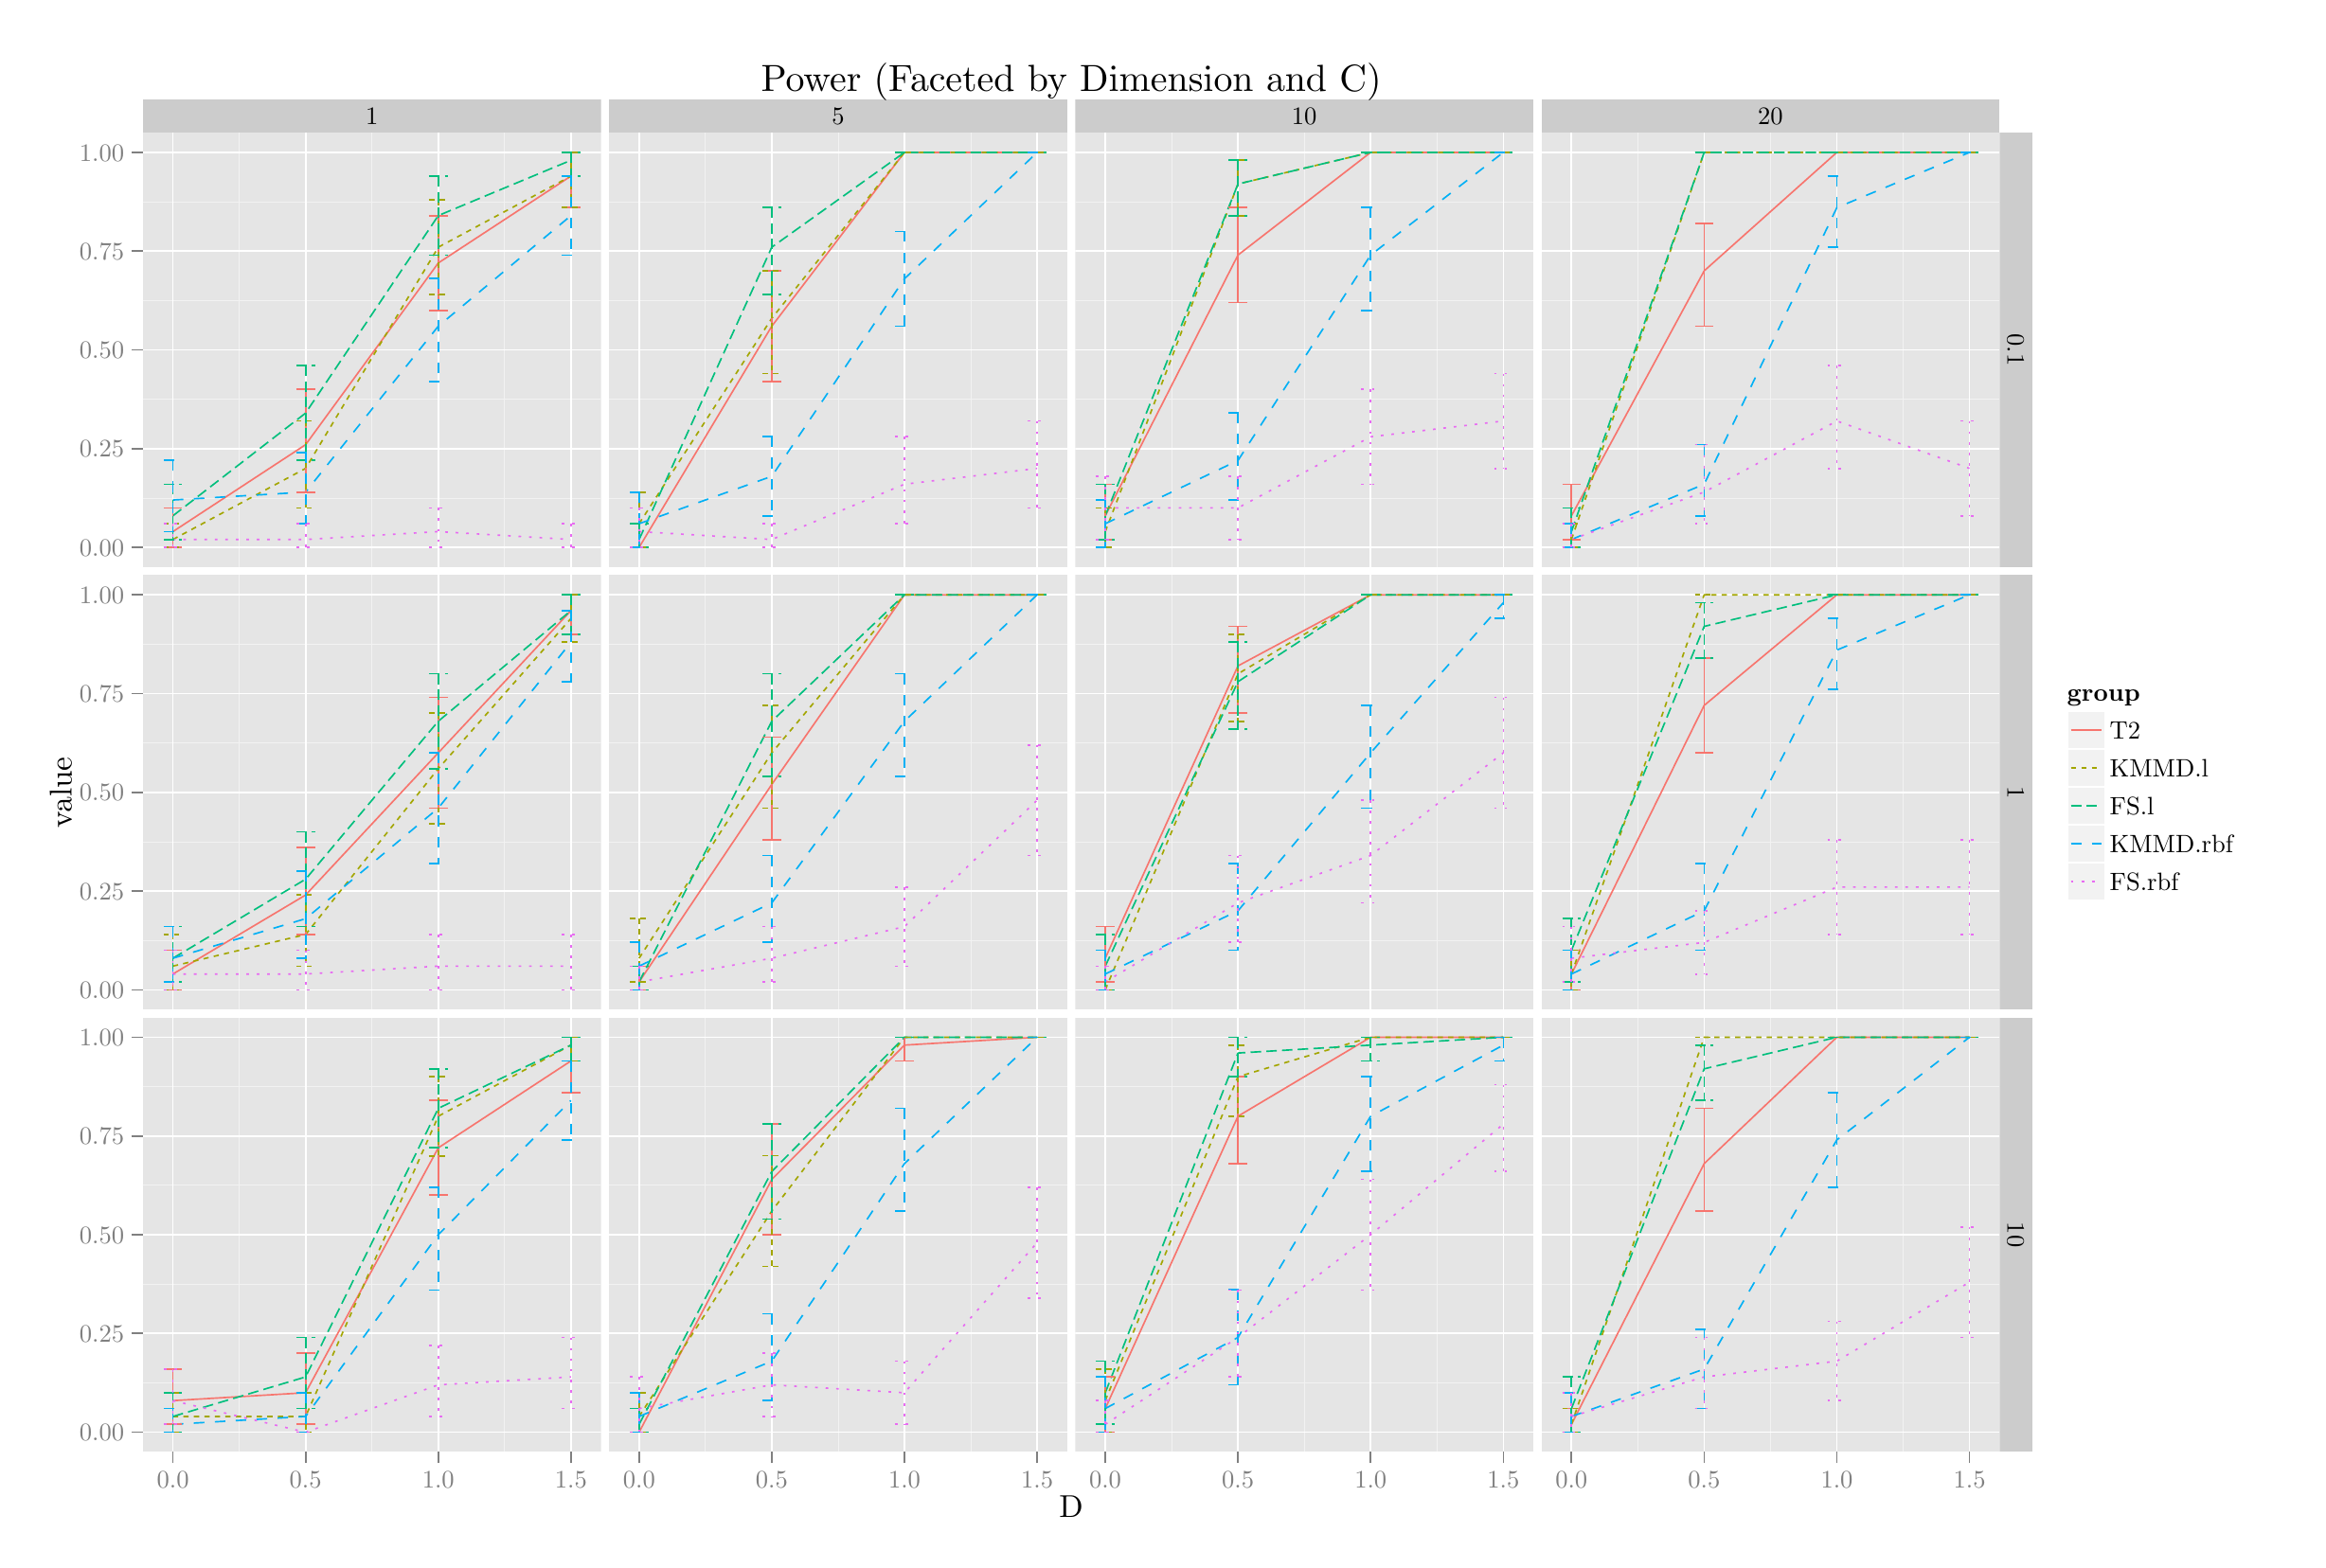
\begin{tikzpicture}[x=1pt,y=1pt]
\definecolor[named]{fillColor}{rgb}{1.00,1.00,1.00}
\path[use as bounding box,fill=fillColor,fill opacity=0.00] (0,0) rectangle (867.24,578.16);
\begin{scope}
\path[clip] (  0.00,  0.00) rectangle (867.24,578.16);
\definecolor[named]{drawColor}{rgb}{1.00,1.00,1.00}
\definecolor[named]{fillColor}{rgb}{1.00,1.00,1.00}

\path[draw=drawColor,line width= 0.6pt,line join=round,line cap=round,fill=fillColor] ( -0.00, -0.00) rectangle (867.24,578.16);
\end{scope}
\begin{scope}
\path[clip] ( 44.49,537.54) rectangle (219.34,550.17);
\definecolor[named]{fillColor}{rgb}{0.80,0.80,0.80}

\path[fill=fillColor] ( 44.49,537.54) rectangle (219.34,550.17);
\definecolor[named]{drawColor}{rgb}{0.00,0.00,0.00}

\node[text=drawColor,anchor=base,inner sep=0pt, outer sep=0pt, scale=  0.96] at (131.91,540.55) {1};
\end{scope}
\begin{scope}
\path[clip] (222.35,537.54) rectangle (397.21,550.17);
\definecolor[named]{fillColor}{rgb}{0.80,0.80,0.80}

\path[fill=fillColor] (222.35,537.54) rectangle (397.21,550.17);
\definecolor[named]{drawColor}{rgb}{0.00,0.00,0.00}

\node[text=drawColor,anchor=base,inner sep=0pt, outer sep=0pt, scale=  0.96] at (309.78,540.55) {5};
\end{scope}
\begin{scope}
\path[clip] (400.22,537.54) rectangle (575.08,550.17);
\definecolor[named]{fillColor}{rgb}{0.80,0.80,0.80}

\path[fill=fillColor] (400.22,537.54) rectangle (575.08,550.17);
\definecolor[named]{drawColor}{rgb}{0.00,0.00,0.00}

\node[text=drawColor,anchor=base,inner sep=0pt, outer sep=0pt, scale=  0.96] at (487.65,540.55) {10};
\end{scope}
\begin{scope}
\path[clip] (578.09,537.54) rectangle (752.95,550.17);
\definecolor[named]{fillColor}{rgb}{0.80,0.80,0.80}

\path[fill=fillColor] (578.09,537.54) rectangle (752.95,550.17);
\definecolor[named]{drawColor}{rgb}{0.00,0.00,0.00}

\node[text=drawColor,anchor=base,inner sep=0pt, outer sep=0pt, scale=  0.96] at (665.52,540.55) {20};
\end{scope}
\begin{scope}
\path[clip] ( 44.49,371.71) rectangle (219.34,537.54);
\definecolor[named]{fillColor}{rgb}{0.90,0.90,0.90}

\path[fill=fillColor] ( 44.49,371.71) rectangle (219.34,537.54);
\definecolor[named]{drawColor}{rgb}{0.95,0.95,0.95}

\path[draw=drawColor,line width= 0.3pt,line join=round] ( 44.49,398.09) --
	(219.34,398.09);

\path[draw=drawColor,line width= 0.3pt,line join=round] ( 44.49,435.78) --
	(219.34,435.78);

\path[draw=drawColor,line width= 0.3pt,line join=round] ( 44.49,473.47) --
	(219.34,473.47);

\path[draw=drawColor,line width= 0.3pt,line join=round] ( 44.49,511.16) --
	(219.34,511.16);

\path[draw=drawColor,line width= 0.3pt,line join=round] ( 81.29,371.71) --
	( 81.29,537.54);

\path[draw=drawColor,line width= 0.3pt,line join=round] (131.91,371.71) --
	(131.91,537.54);

\path[draw=drawColor,line width= 0.3pt,line join=round] (182.54,371.71) --
	(182.54,537.54);
\definecolor[named]{drawColor}{rgb}{1.00,1.00,1.00}

\path[draw=drawColor,line width= 0.6pt,line join=round] ( 44.49,379.25) --
	(219.34,379.25);

\path[draw=drawColor,line width= 0.6pt,line join=round] ( 44.49,416.94) --
	(219.34,416.94);

\path[draw=drawColor,line width= 0.6pt,line join=round] ( 44.49,454.63) --
	(219.34,454.63);

\path[draw=drawColor,line width= 0.6pt,line join=round] ( 44.49,492.31) --
	(219.34,492.31);

\path[draw=drawColor,line width= 0.6pt,line join=round] ( 44.49,530.00) --
	(219.34,530.00);

\path[draw=drawColor,line width= 0.6pt,line join=round] ( 55.98,371.71) --
	( 55.98,537.54);

\path[draw=drawColor,line width= 0.6pt,line join=round] (106.60,371.71) --
	(106.60,537.54);

\path[draw=drawColor,line width= 0.6pt,line join=round] (157.23,371.71) --
	(157.23,537.54);

\path[draw=drawColor,line width= 0.6pt,line join=round] (207.85,371.71) --
	(207.85,537.54);
\definecolor[named]{drawColor}{rgb}{0.97,0.46,0.43}

\path[draw=drawColor,line width= 0.6pt,line join=round] ( 55.98,385.28) --
	(106.60,418.45) --
	(157.23,487.79) --
	(207.85,520.96);
\definecolor[named]{drawColor}{rgb}{0.64,0.65,0.00}

\path[draw=drawColor,line width= 0.6pt,dash pattern=on 2pt off 2pt ,line join=round] ( 55.98,382.27) --
	(106.60,409.40) --
	(157.23,493.82) --
	(207.85,520.96);
\definecolor[named]{drawColor}{rgb}{0.00,0.75,0.49}

\path[draw=drawColor,line width= 0.6pt,dash pattern=on 4pt off 2pt ,line join=round] ( 55.98,391.31) --
	(106.60,430.51) --
	(157.23,505.88) --
	(207.85,526.99);
\definecolor[named]{drawColor}{rgb}{0.00,0.69,0.96}

\path[draw=drawColor,line width= 0.6pt,dash pattern=on 4pt off 4pt ,line join=round] ( 55.98,397.34) --
	(106.60,400.36) --
	(157.23,463.67) --
	(207.85,505.88);
\definecolor[named]{drawColor}{rgb}{0.91,0.42,0.95}

\path[draw=drawColor,line width= 0.6pt,dash pattern=on 1pt off 3pt ,line join=round] ( 55.98,382.27) --
	(106.60,382.27) --
	(157.23,385.28) --
	(207.85,382.27);
\definecolor[named]{drawColor}{rgb}{0.97,0.46,0.43}

\path[draw=drawColor,line width= 0.6pt,line join=round] ( 52.43,394.33) --
	( 59.52,394.33);

\path[draw=drawColor,line width= 0.6pt,line join=round] ( 55.98,394.33) --
	( 55.98,379.25);

\path[draw=drawColor,line width= 0.6pt,line join=round] ( 52.43,379.25) --
	( 59.52,379.25);

\path[draw=drawColor,line width= 0.6pt,line join=round] (103.06,439.55) --
	(110.15,439.55);

\path[draw=drawColor,line width= 0.6pt,line join=round] (106.60,439.55) --
	(106.60,400.36);

\path[draw=drawColor,line width= 0.6pt,line join=round] (103.06,400.36) --
	(110.15,400.36);

\path[draw=drawColor,line width= 0.6pt,line join=round] (153.68,505.88) --
	(160.77,505.88);

\path[draw=drawColor,line width= 0.6pt,line join=round] (157.23,505.88) --
	(157.23,469.70);

\path[draw=drawColor,line width= 0.6pt,line join=round] (153.68,469.70) --
	(160.77,469.70);

\path[draw=drawColor,line width= 0.6pt,line join=round] (204.31,530.00) --
	(211.39,530.00);

\path[draw=drawColor,line width= 0.6pt,line join=round] (207.85,530.00) --
	(207.85,508.90);

\path[draw=drawColor,line width= 0.6pt,line join=round] (204.31,508.90) --
	(211.39,508.90);
\definecolor[named]{drawColor}{rgb}{0.64,0.65,0.00}

\path[draw=drawColor,line width= 0.6pt,dash pattern=on 2pt off 2pt ,line join=round] ( 52.43,388.30) --
	( 59.52,388.30);

\path[draw=drawColor,line width= 0.6pt,dash pattern=on 2pt off 2pt ,line join=round] ( 55.98,388.30) --
	( 55.98,379.25);

\path[draw=drawColor,line width= 0.6pt,dash pattern=on 2pt off 2pt ,line join=round] ( 52.43,379.25) --
	( 59.52,379.25);

\path[draw=drawColor,line width= 0.6pt,dash pattern=on 2pt off 2pt ,line join=round] (103.06,427.49) --
	(110.15,427.49);

\path[draw=drawColor,line width= 0.6pt,dash pattern=on 2pt off 2pt ,line join=round] (106.60,427.49) --
	(106.60,394.33);

\path[draw=drawColor,line width= 0.6pt,dash pattern=on 2pt off 2pt ,line join=round] (103.06,394.33) --
	(110.15,394.33);

\path[draw=drawColor,line width= 0.6pt,dash pattern=on 2pt off 2pt ,line join=round] (153.68,511.91) --
	(160.77,511.91);

\path[draw=drawColor,line width= 0.6pt,dash pattern=on 2pt off 2pt ,line join=round] (157.23,511.91) --
	(157.23,475.73);

\path[draw=drawColor,line width= 0.6pt,dash pattern=on 2pt off 2pt ,line join=round] (153.68,475.73) --
	(160.77,475.73);

\path[draw=drawColor,line width= 0.6pt,dash pattern=on 2pt off 2pt ,line join=round] (204.31,530.00) --
	(211.39,530.00);

\path[draw=drawColor,line width= 0.6pt,dash pattern=on 2pt off 2pt ,line join=round] (207.85,530.00) --
	(207.85,508.90);

\path[draw=drawColor,line width= 0.6pt,dash pattern=on 2pt off 2pt ,line join=round] (204.31,508.90) --
	(211.39,508.90);
\definecolor[named]{drawColor}{rgb}{0.00,0.75,0.49}

\path[draw=drawColor,line width= 0.6pt,dash pattern=on 4pt off 2pt ,line join=round] ( 52.43,403.37) --
	( 59.52,403.37);

\path[draw=drawColor,line width= 0.6pt,dash pattern=on 4pt off 2pt ,line join=round] ( 55.98,403.37) --
	( 55.98,382.27);

\path[draw=drawColor,line width= 0.6pt,dash pattern=on 4pt off 2pt ,line join=round] ( 52.43,382.27) --
	( 59.52,382.27);

\path[draw=drawColor,line width= 0.6pt,dash pattern=on 4pt off 2pt ,line join=round] (103.06,448.67) --
	(110.15,448.67);

\path[draw=drawColor,line width= 0.6pt,dash pattern=on 4pt off 2pt ,line join=round] (106.60,448.67) --
	(106.60,412.42);

\path[draw=drawColor,line width= 0.6pt,dash pattern=on 4pt off 2pt ,line join=round] (103.06,412.42) --
	(110.15,412.42);

\path[draw=drawColor,line width= 0.6pt,dash pattern=on 4pt off 2pt ,line join=round] (153.68,520.96) --
	(160.77,520.96);

\path[draw=drawColor,line width= 0.6pt,dash pattern=on 4pt off 2pt ,line join=round] (157.23,520.96) --
	(157.23,490.73);

\path[draw=drawColor,line width= 0.6pt,dash pattern=on 4pt off 2pt ,line join=round] (153.68,490.73) --
	(160.77,490.73);

\path[draw=drawColor,line width= 0.6pt,dash pattern=on 4pt off 2pt ,line join=round] (204.31,530.00) --
	(211.39,530.00);

\path[draw=drawColor,line width= 0.6pt,dash pattern=on 4pt off 2pt ,line join=round] (207.85,530.00) --
	(207.85,520.96);

\path[draw=drawColor,line width= 0.6pt,dash pattern=on 4pt off 2pt ,line join=round] (204.31,520.96) --
	(211.39,520.96);
\definecolor[named]{drawColor}{rgb}{0.00,0.69,0.96}

\path[draw=drawColor,line width= 0.6pt,dash pattern=on 4pt off 4pt ,line join=round] ( 52.43,412.42) --
	( 59.52,412.42);

\path[draw=drawColor,line width= 0.6pt,dash pattern=on 4pt off 4pt ,line join=round] ( 55.98,412.42) --
	( 55.98,385.28);

\path[draw=drawColor,line width= 0.6pt,dash pattern=on 4pt off 4pt ,line join=round] ( 52.43,385.28) --
	( 59.52,385.28);

\path[draw=drawColor,line width= 0.6pt,dash pattern=on 4pt off 4pt ,line join=round] (103.06,415.43) --
	(110.15,415.43);

\path[draw=drawColor,line width= 0.6pt,dash pattern=on 4pt off 4pt ,line join=round] (106.60,415.43) --
	(106.60,388.30);

\path[draw=drawColor,line width= 0.6pt,dash pattern=on 4pt off 4pt ,line join=round] (103.06,388.30) --
	(110.15,388.30);

\path[draw=drawColor,line width= 0.6pt,dash pattern=on 4pt off 4pt ,line join=round] (153.68,481.84) --
	(160.77,481.84);

\path[draw=drawColor,line width= 0.6pt,dash pattern=on 4pt off 4pt ,line join=round] (157.23,481.84) --
	(157.23,442.57);

\path[draw=drawColor,line width= 0.6pt,dash pattern=on 4pt off 4pt ,line join=round] (153.68,442.57) --
	(160.77,442.57);

\path[draw=drawColor,line width= 0.6pt,dash pattern=on 4pt off 4pt ,line join=round] (204.31,520.96) --
	(211.39,520.96);

\path[draw=drawColor,line width= 0.6pt,dash pattern=on 4pt off 4pt ,line join=round] (207.85,520.96) --
	(207.85,490.81);

\path[draw=drawColor,line width= 0.6pt,dash pattern=on 4pt off 4pt ,line join=round] (204.31,490.81) --
	(211.39,490.81);
\definecolor[named]{drawColor}{rgb}{0.91,0.42,0.95}

\path[draw=drawColor,line width= 0.6pt,dash pattern=on 1pt off 3pt ,line join=round] ( 52.43,388.30) --
	( 59.52,388.30);

\path[draw=drawColor,line width= 0.6pt,dash pattern=on 1pt off 3pt ,line join=round] ( 55.98,388.30) --
	( 55.98,379.25);

\path[draw=drawColor,line width= 0.6pt,dash pattern=on 1pt off 3pt ,line join=round] ( 52.43,379.25) --
	( 59.52,379.25);

\path[draw=drawColor,line width= 0.6pt,dash pattern=on 1pt off 3pt ,line join=round] (103.06,388.30) --
	(110.15,388.30);

\path[draw=drawColor,line width= 0.6pt,dash pattern=on 1pt off 3pt ,line join=round] (106.60,388.30) --
	(106.60,379.25);

\path[draw=drawColor,line width= 0.6pt,dash pattern=on 1pt off 3pt ,line join=round] (103.06,379.25) --
	(110.15,379.25);

\path[draw=drawColor,line width= 0.6pt,dash pattern=on 1pt off 3pt ,line join=round] (153.68,394.33) --
	(160.77,394.33);

\path[draw=drawColor,line width= 0.6pt,dash pattern=on 1pt off 3pt ,line join=round] (157.23,394.33) --
	(157.23,379.25);

\path[draw=drawColor,line width= 0.6pt,dash pattern=on 1pt off 3pt ,line join=round] (153.68,379.25) --
	(160.77,379.25);

\path[draw=drawColor,line width= 0.6pt,dash pattern=on 1pt off 3pt ,line join=round] (204.31,388.30) --
	(211.39,388.30);

\path[draw=drawColor,line width= 0.6pt,dash pattern=on 1pt off 3pt ,line join=round] (207.85,388.30) --
	(207.85,379.25);

\path[draw=drawColor,line width= 0.6pt,dash pattern=on 1pt off 3pt ,line join=round] (204.31,379.25) --
	(211.39,379.25);
\end{scope}
\begin{scope}
\path[clip] ( 44.49,202.87) rectangle (219.34,368.70);
\definecolor[named]{fillColor}{rgb}{0.90,0.90,0.90}

\path[fill=fillColor] ( 44.49,202.87) rectangle (219.34,368.70);
\definecolor[named]{drawColor}{rgb}{0.95,0.95,0.95}

\path[draw=drawColor,line width= 0.3pt,line join=round] ( 44.49,229.26) --
	(219.34,229.26);

\path[draw=drawColor,line width= 0.3pt,line join=round] ( 44.49,266.94) --
	(219.34,266.94);

\path[draw=drawColor,line width= 0.3pt,line join=round] ( 44.49,304.63) --
	(219.34,304.63);

\path[draw=drawColor,line width= 0.3pt,line join=round] ( 44.49,342.32) --
	(219.34,342.32);

\path[draw=drawColor,line width= 0.3pt,line join=round] ( 81.29,202.87) --
	( 81.29,368.70);

\path[draw=drawColor,line width= 0.3pt,line join=round] (131.91,202.87) --
	(131.91,368.70);

\path[draw=drawColor,line width= 0.3pt,line join=round] (182.54,202.87) --
	(182.54,368.70);
\definecolor[named]{drawColor}{rgb}{1.00,1.00,1.00}

\path[draw=drawColor,line width= 0.6pt,line join=round] ( 44.49,210.41) --
	(219.34,210.41);

\path[draw=drawColor,line width= 0.6pt,line join=round] ( 44.49,248.10) --
	(219.34,248.10);

\path[draw=drawColor,line width= 0.6pt,line join=round] ( 44.49,285.79) --
	(219.34,285.79);

\path[draw=drawColor,line width= 0.6pt,line join=round] ( 44.49,323.48) --
	(219.34,323.48);

\path[draw=drawColor,line width= 0.6pt,line join=round] ( 44.49,361.16) --
	(219.34,361.16);

\path[draw=drawColor,line width= 0.6pt,line join=round] ( 55.98,202.87) --
	( 55.98,368.70);

\path[draw=drawColor,line width= 0.6pt,line join=round] (106.60,202.87) --
	(106.60,368.70);

\path[draw=drawColor,line width= 0.6pt,line join=round] (157.23,202.87) --
	(157.23,368.70);

\path[draw=drawColor,line width= 0.6pt,line join=round] (207.85,202.87) --
	(207.85,368.70);
\definecolor[named]{drawColor}{rgb}{0.97,0.46,0.43}

\path[draw=drawColor,line width= 0.6pt,line join=round] ( 55.98,216.44) --
	(106.60,246.59) --
	(157.23,300.86) --
	(207.85,355.13);
\definecolor[named]{drawColor}{rgb}{0.64,0.65,0.00}

\path[draw=drawColor,line width= 0.6pt,dash pattern=on 2pt off 2pt ,line join=round] ( 55.98,219.46) --
	(106.60,231.52) --
	(157.23,294.83) --
	(207.85,352.12);
\definecolor[named]{drawColor}{rgb}{0.00,0.75,0.49}

\path[draw=drawColor,line width= 0.6pt,dash pattern=on 4pt off 2pt ,line join=round] ( 55.98,222.47) --
	(106.60,252.62) --
	(157.23,312.92) --
	(207.85,355.13);
\definecolor[named]{drawColor}{rgb}{0.00,0.69,0.96}

\path[draw=drawColor,line width= 0.6pt,dash pattern=on 4pt off 4pt ,line join=round] ( 55.98,222.47) --
	(106.60,237.55) --
	(157.23,279.76) --
	(207.85,343.07);
\definecolor[named]{drawColor}{rgb}{0.91,0.42,0.95}

\path[draw=drawColor,line width= 0.6pt,dash pattern=on 1pt off 3pt ,line join=round] ( 55.98,216.44) --
	(106.60,216.44) --
	(157.23,219.46) --
	(207.85,219.46);
\definecolor[named]{drawColor}{rgb}{0.97,0.46,0.43}

\path[draw=drawColor,line width= 0.6pt,line join=round] ( 52.43,225.49) --
	( 59.52,225.49);

\path[draw=drawColor,line width= 0.6pt,line join=round] ( 55.98,225.49) --
	( 55.98,210.41);

\path[draw=drawColor,line width= 0.6pt,line join=round] ( 52.43,210.41) --
	( 59.52,210.41);

\path[draw=drawColor,line width= 0.6pt,line join=round] (103.06,264.68) --
	(110.15,264.68);

\path[draw=drawColor,line width= 0.6pt,line join=round] (106.60,264.68) --
	(106.60,231.52);

\path[draw=drawColor,line width= 0.6pt,line join=round] (103.06,231.52) --
	(110.15,231.52);

\path[draw=drawColor,line width= 0.6pt,line join=round] (153.68,321.97) --
	(160.77,321.97);

\path[draw=drawColor,line width= 0.6pt,line join=round] (157.23,321.97) --
	(157.23,279.76);

\path[draw=drawColor,line width= 0.6pt,line join=round] (153.68,279.76) --
	(160.77,279.76);

\path[draw=drawColor,line width= 0.6pt,line join=round] (204.31,361.16) --
	(211.39,361.16);

\path[draw=drawColor,line width= 0.6pt,line join=round] (207.85,361.16) --
	(207.85,346.09);

\path[draw=drawColor,line width= 0.6pt,line join=round] (204.31,346.09) --
	(211.39,346.09);
\definecolor[named]{drawColor}{rgb}{0.64,0.65,0.00}

\path[draw=drawColor,line width= 0.6pt,dash pattern=on 2pt off 2pt ,line join=round] ( 52.43,231.52) --
	( 59.52,231.52);

\path[draw=drawColor,line width= 0.6pt,dash pattern=on 2pt off 2pt ,line join=round] ( 55.98,231.52) --
	( 55.98,210.41);

\path[draw=drawColor,line width= 0.6pt,dash pattern=on 2pt off 2pt ,line join=round] ( 52.43,210.41) --
	( 59.52,210.41);

\path[draw=drawColor,line width= 0.6pt,dash pattern=on 2pt off 2pt ,line join=round] (103.06,246.59) --
	(110.15,246.59);

\path[draw=drawColor,line width= 0.6pt,dash pattern=on 2pt off 2pt ,line join=round] (106.60,246.59) --
	(106.60,219.38);

\path[draw=drawColor,line width= 0.6pt,dash pattern=on 2pt off 2pt ,line join=round] (103.06,219.38) --
	(110.15,219.38);

\path[draw=drawColor,line width= 0.6pt,dash pattern=on 2pt off 2pt ,line join=round] (153.68,315.94) --
	(160.77,315.94);

\path[draw=drawColor,line width= 0.6pt,dash pattern=on 2pt off 2pt ,line join=round] (157.23,315.94) --
	(157.23,273.73);

\path[draw=drawColor,line width= 0.6pt,dash pattern=on 2pt off 2pt ,line join=round] (153.68,273.73) --
	(160.77,273.73);

\path[draw=drawColor,line width= 0.6pt,dash pattern=on 2pt off 2pt ,line join=round] (204.31,361.16) --
	(211.39,361.16);

\path[draw=drawColor,line width= 0.6pt,dash pattern=on 2pt off 2pt ,line join=round] (207.85,361.16) --
	(207.85,343.07);

\path[draw=drawColor,line width= 0.6pt,dash pattern=on 2pt off 2pt ,line join=round] (204.31,343.07) --
	(211.39,343.07);
\definecolor[named]{drawColor}{rgb}{0.00,0.75,0.49}

\path[draw=drawColor,line width= 0.6pt,dash pattern=on 4pt off 2pt ,line join=round] ( 52.43,234.53) --
	( 59.52,234.53);

\path[draw=drawColor,line width= 0.6pt,dash pattern=on 4pt off 2pt ,line join=round] ( 55.98,234.53) --
	( 55.98,213.43);

\path[draw=drawColor,line width= 0.6pt,dash pattern=on 4pt off 2pt ,line join=round] ( 52.43,213.43) --
	( 59.52,213.43);

\path[draw=drawColor,line width= 0.6pt,dash pattern=on 4pt off 2pt ,line join=round] (103.06,270.71) --
	(110.15,270.71);

\path[draw=drawColor,line width= 0.6pt,dash pattern=on 4pt off 2pt ,line join=round] (106.60,270.71) --
	(106.60,234.53);

\path[draw=drawColor,line width= 0.6pt,dash pattern=on 4pt off 2pt ,line join=round] (103.06,234.53) --
	(110.15,234.53);

\path[draw=drawColor,line width= 0.6pt,dash pattern=on 4pt off 2pt ,line join=round] (153.68,331.01) --
	(160.77,331.01);

\path[draw=drawColor,line width= 0.6pt,dash pattern=on 4pt off 2pt ,line join=round] (157.23,331.01) --
	(157.23,294.83);

\path[draw=drawColor,line width= 0.6pt,dash pattern=on 4pt off 2pt ,line join=round] (153.68,294.83) --
	(160.77,294.83);

\path[draw=drawColor,line width= 0.6pt,dash pattern=on 4pt off 2pt ,line join=round] (204.31,361.16) --
	(211.39,361.16);

\path[draw=drawColor,line width= 0.6pt,dash pattern=on 4pt off 2pt ,line join=round] (207.85,361.16) --
	(207.85,346.09);

\path[draw=drawColor,line width= 0.6pt,dash pattern=on 4pt off 2pt ,line join=round] (204.31,346.09) --
	(211.39,346.09);
\definecolor[named]{drawColor}{rgb}{0.00,0.69,0.96}

\path[draw=drawColor,line width= 0.6pt,dash pattern=on 4pt off 4pt ,line join=round] ( 52.43,234.53) --
	( 59.52,234.53);

\path[draw=drawColor,line width= 0.6pt,dash pattern=on 4pt off 4pt ,line join=round] ( 55.98,234.53) --
	( 55.98,213.43);

\path[draw=drawColor,line width= 0.6pt,dash pattern=on 4pt off 4pt ,line join=round] ( 52.43,213.43) --
	( 59.52,213.43);

\path[draw=drawColor,line width= 0.6pt,dash pattern=on 4pt off 4pt ,line join=round] (103.06,255.64) --
	(110.15,255.64);

\path[draw=drawColor,line width= 0.6pt,dash pattern=on 4pt off 4pt ,line join=round] (106.60,255.64) --
	(106.60,222.47);

\path[draw=drawColor,line width= 0.6pt,dash pattern=on 4pt off 4pt ,line join=round] (103.06,222.47) --
	(110.15,222.47);

\path[draw=drawColor,line width= 0.6pt,dash pattern=on 4pt off 4pt ,line join=round] (153.68,300.86) --
	(160.77,300.86);

\path[draw=drawColor,line width= 0.6pt,dash pattern=on 4pt off 4pt ,line join=round] (157.23,300.86) --
	(157.23,258.65);

\path[draw=drawColor,line width= 0.6pt,dash pattern=on 4pt off 4pt ,line join=round] (153.68,258.65) --
	(160.77,258.65);

\path[draw=drawColor,line width= 0.6pt,dash pattern=on 4pt off 4pt ,line join=round] (204.31,355.13) --
	(211.39,355.13);

\path[draw=drawColor,line width= 0.6pt,dash pattern=on 4pt off 4pt ,line join=round] (207.85,355.13) --
	(207.85,328.00);

\path[draw=drawColor,line width= 0.6pt,dash pattern=on 4pt off 4pt ,line join=round] (204.31,328.00) --
	(211.39,328.00);
\definecolor[named]{drawColor}{rgb}{0.91,0.42,0.95}

\path[draw=drawColor,line width= 0.6pt,dash pattern=on 1pt off 3pt ,line join=round] ( 52.43,225.49) --
	( 59.52,225.49);

\path[draw=drawColor,line width= 0.6pt,dash pattern=on 1pt off 3pt ,line join=round] ( 55.98,225.49) --
	( 55.98,210.41);

\path[draw=drawColor,line width= 0.6pt,dash pattern=on 1pt off 3pt ,line join=round] ( 52.43,210.41) --
	( 59.52,210.41);

\path[draw=drawColor,line width= 0.6pt,dash pattern=on 1pt off 3pt ,line join=round] (103.06,225.49) --
	(110.15,225.49);

\path[draw=drawColor,line width= 0.6pt,dash pattern=on 1pt off 3pt ,line join=round] (106.60,225.49) --
	(106.60,210.41);

\path[draw=drawColor,line width= 0.6pt,dash pattern=on 1pt off 3pt ,line join=round] (103.06,210.41) --
	(110.15,210.41);

\path[draw=drawColor,line width= 0.6pt,dash pattern=on 1pt off 3pt ,line join=round] (153.68,231.52) --
	(160.77,231.52);

\path[draw=drawColor,line width= 0.6pt,dash pattern=on 1pt off 3pt ,line join=round] (157.23,231.52) --
	(157.23,210.41);

\path[draw=drawColor,line width= 0.6pt,dash pattern=on 1pt off 3pt ,line join=round] (153.68,210.41) --
	(160.77,210.41);

\path[draw=drawColor,line width= 0.6pt,dash pattern=on 1pt off 3pt ,line join=round] (204.31,231.52) --
	(211.39,231.52);

\path[draw=drawColor,line width= 0.6pt,dash pattern=on 1pt off 3pt ,line join=round] (207.85,231.52) --
	(207.85,210.41);

\path[draw=drawColor,line width= 0.6pt,dash pattern=on 1pt off 3pt ,line join=round] (204.31,210.41) --
	(211.39,210.41);
\end{scope}
\begin{scope}
\path[clip] ( 44.49, 34.03) rectangle (219.34,199.86);
\definecolor[named]{fillColor}{rgb}{0.90,0.90,0.90}

\path[fill=fillColor] ( 44.49, 34.03) rectangle (219.34,199.86);
\definecolor[named]{drawColor}{rgb}{0.95,0.95,0.95}

\path[draw=drawColor,line width= 0.3pt,line join=round] ( 44.49, 60.42) --
	(219.34, 60.42);

\path[draw=drawColor,line width= 0.3pt,line join=round] ( 44.49, 98.10) --
	(219.34, 98.10);

\path[draw=drawColor,line width= 0.3pt,line join=round] ( 44.49,135.79) --
	(219.34,135.79);

\path[draw=drawColor,line width= 0.3pt,line join=round] ( 44.49,173.48) --
	(219.34,173.48);

\path[draw=drawColor,line width= 0.3pt,line join=round] ( 81.29, 34.03) --
	( 81.29,199.86);

\path[draw=drawColor,line width= 0.3pt,line join=round] (131.91, 34.03) --
	(131.91,199.86);

\path[draw=drawColor,line width= 0.3pt,line join=round] (182.54, 34.03) --
	(182.54,199.86);
\definecolor[named]{drawColor}{rgb}{1.00,1.00,1.00}

\path[draw=drawColor,line width= 0.6pt,line join=round] ( 44.49, 41.57) --
	(219.34, 41.57);

\path[draw=drawColor,line width= 0.6pt,line join=round] ( 44.49, 79.26) --
	(219.34, 79.26);

\path[draw=drawColor,line width= 0.6pt,line join=round] ( 44.49,116.95) --
	(219.34,116.95);

\path[draw=drawColor,line width= 0.6pt,line join=round] ( 44.49,154.64) --
	(219.34,154.64);

\path[draw=drawColor,line width= 0.6pt,line join=round] ( 44.49,192.32) --
	(219.34,192.32);

\path[draw=drawColor,line width= 0.6pt,line join=round] ( 55.98, 34.03) --
	( 55.98,199.86);

\path[draw=drawColor,line width= 0.6pt,line join=round] (106.60, 34.03) --
	(106.60,199.86);

\path[draw=drawColor,line width= 0.6pt,line join=round] (157.23, 34.03) --
	(157.23,199.86);

\path[draw=drawColor,line width= 0.6pt,line join=round] (207.85, 34.03) --
	(207.85,199.86);
\definecolor[named]{drawColor}{rgb}{0.97,0.46,0.43}

\path[draw=drawColor,line width= 0.6pt,line join=round] ( 55.98, 53.63) --
	(106.60, 56.65) --
	(157.23,150.11) --
	(207.85,183.28);
\definecolor[named]{drawColor}{rgb}{0.64,0.65,0.00}

\path[draw=drawColor,line width= 0.6pt,dash pattern=on 2pt off 2pt ,line join=round] ( 55.98, 47.60) --
	(106.60, 47.60) --
	(157.23,162.17) --
	(207.85,189.31);
\definecolor[named]{drawColor}{rgb}{0.00,0.75,0.49}

\path[draw=drawColor,line width= 0.6pt,dash pattern=on 4pt off 2pt ,line join=round] ( 55.98, 47.60) --
	(106.60, 62.68) --
	(157.23,165.19) --
	(207.85,189.31);
\definecolor[named]{drawColor}{rgb}{0.00,0.69,0.96}

\path[draw=drawColor,line width= 0.6pt,dash pattern=on 4pt off 4pt ,line join=round] ( 55.98, 44.59) --
	(106.60, 47.60) --
	(157.23,116.95) --
	(207.85,168.20);
\definecolor[named]{drawColor}{rgb}{0.91,0.42,0.95}

\path[draw=drawColor,line width= 0.6pt,dash pattern=on 1pt off 3pt ,line join=round] ( 55.98, 53.63) --
	(106.60, 41.57) --
	(157.23, 59.66) --
	(207.85, 62.68);
\definecolor[named]{drawColor}{rgb}{0.97,0.46,0.43}

\path[draw=drawColor,line width= 0.6pt,line join=round] ( 52.43, 65.69) --
	( 59.52, 65.69);

\path[draw=drawColor,line width= 0.6pt,line join=round] ( 55.98, 65.69) --
	( 55.98, 44.59);

\path[draw=drawColor,line width= 0.6pt,line join=round] ( 52.43, 44.59) --
	( 59.52, 44.59);

\path[draw=drawColor,line width= 0.6pt,line join=round] (103.06, 71.72) --
	(110.15, 71.72);

\path[draw=drawColor,line width= 0.6pt,line join=round] (106.60, 71.72) --
	(106.60, 44.59);

\path[draw=drawColor,line width= 0.6pt,line join=round] (103.06, 44.59) --
	(110.15, 44.59);

\path[draw=drawColor,line width= 0.6pt,line join=round] (153.68,168.20) --
	(160.77,168.20);

\path[draw=drawColor,line width= 0.6pt,line join=round] (157.23,168.20) --
	(157.23,132.02);

\path[draw=drawColor,line width= 0.6pt,line join=round] (153.68,132.02) --
	(160.77,132.02);

\path[draw=drawColor,line width= 0.6pt,line join=round] (204.31,192.32) --
	(211.39,192.32);

\path[draw=drawColor,line width= 0.6pt,line join=round] (207.85,192.32) --
	(207.85,171.22);

\path[draw=drawColor,line width= 0.6pt,line join=round] (204.31,171.22) --
	(211.39,171.22);
\definecolor[named]{drawColor}{rgb}{0.64,0.65,0.00}

\path[draw=drawColor,line width= 0.6pt,dash pattern=on 2pt off 2pt ,line join=round] ( 52.43, 56.65) --
	( 59.52, 56.65);

\path[draw=drawColor,line width= 0.6pt,dash pattern=on 2pt off 2pt ,line join=round] ( 55.98, 56.65) --
	( 55.98, 41.57);

\path[draw=drawColor,line width= 0.6pt,dash pattern=on 2pt off 2pt ,line join=round] ( 52.43, 41.57) --
	( 59.52, 41.57);

\path[draw=drawColor,line width= 0.6pt,dash pattern=on 2pt off 2pt ,line join=round] (103.06, 56.65) --
	(110.15, 56.65);

\path[draw=drawColor,line width= 0.6pt,dash pattern=on 2pt off 2pt ,line join=round] (106.60, 56.65) --
	(106.60, 41.57);

\path[draw=drawColor,line width= 0.6pt,dash pattern=on 2pt off 2pt ,line join=round] (103.06, 41.57) --
	(110.15, 41.57);

\path[draw=drawColor,line width= 0.6pt,dash pattern=on 2pt off 2pt ,line join=round] (153.68,177.25) --
	(160.77,177.25);

\path[draw=drawColor,line width= 0.6pt,dash pattern=on 2pt off 2pt ,line join=round] (157.23,177.25) --
	(157.23,147.02);

\path[draw=drawColor,line width= 0.6pt,dash pattern=on 2pt off 2pt ,line join=round] (153.68,147.02) --
	(160.77,147.02);

\path[draw=drawColor,line width= 0.6pt,dash pattern=on 2pt off 2pt ,line join=round] (204.31,192.32) --
	(211.39,192.32);

\path[draw=drawColor,line width= 0.6pt,dash pattern=on 2pt off 2pt ,line join=round] (207.85,192.32) --
	(207.85,183.28);

\path[draw=drawColor,line width= 0.6pt,dash pattern=on 2pt off 2pt ,line join=round] (204.31,183.28) --
	(211.39,183.28);
\definecolor[named]{drawColor}{rgb}{0.00,0.75,0.49}

\path[draw=drawColor,line width= 0.6pt,dash pattern=on 4pt off 2pt ,line join=round] ( 52.43, 56.65) --
	( 59.52, 56.65);

\path[draw=drawColor,line width= 0.6pt,dash pattern=on 4pt off 2pt ,line join=round] ( 55.98, 56.65) --
	( 55.98, 41.57);

\path[draw=drawColor,line width= 0.6pt,dash pattern=on 4pt off 2pt ,line join=round] ( 52.43, 41.57) --
	( 59.52, 41.57);

\path[draw=drawColor,line width= 0.6pt,dash pattern=on 4pt off 2pt ,line join=round] (103.06, 77.75) --
	(110.15, 77.75);

\path[draw=drawColor,line width= 0.6pt,dash pattern=on 4pt off 2pt ,line join=round] (106.60, 77.75) --
	(106.60, 50.62);

\path[draw=drawColor,line width= 0.6pt,dash pattern=on 4pt off 2pt ,line join=round] (103.06, 50.62) --
	(110.15, 50.62);

\path[draw=drawColor,line width= 0.6pt,dash pattern=on 4pt off 2pt ,line join=round] (153.68,180.26) --
	(160.77,180.26);

\path[draw=drawColor,line width= 0.6pt,dash pattern=on 4pt off 2pt ,line join=round] (157.23,180.26) --
	(157.23,150.11);

\path[draw=drawColor,line width= 0.6pt,dash pattern=on 4pt off 2pt ,line join=round] (153.68,150.11) --
	(160.77,150.11);

\path[draw=drawColor,line width= 0.6pt,dash pattern=on 4pt off 2pt ,line join=round] (204.31,192.32) --
	(211.39,192.32);

\path[draw=drawColor,line width= 0.6pt,dash pattern=on 4pt off 2pt ,line join=round] (207.85,192.32) --
	(207.85,183.28);

\path[draw=drawColor,line width= 0.6pt,dash pattern=on 4pt off 2pt ,line join=round] (204.31,183.28) --
	(211.39,183.28);
\definecolor[named]{drawColor}{rgb}{0.00,0.69,0.96}

\path[draw=drawColor,line width= 0.6pt,dash pattern=on 4pt off 4pt ,line join=round] ( 52.43, 50.62) --
	( 59.52, 50.62);

\path[draw=drawColor,line width= 0.6pt,dash pattern=on 4pt off 4pt ,line join=round] ( 55.98, 50.62) --
	( 55.98, 41.57);

\path[draw=drawColor,line width= 0.6pt,dash pattern=on 4pt off 4pt ,line join=round] ( 52.43, 41.57) --
	( 59.52, 41.57);

\path[draw=drawColor,line width= 0.6pt,dash pattern=on 4pt off 4pt ,line join=round] (103.06, 56.65) --
	(110.15, 56.65);

\path[draw=drawColor,line width= 0.6pt,dash pattern=on 4pt off 4pt ,line join=round] (106.60, 56.65) --
	(106.60, 41.57);

\path[draw=drawColor,line width= 0.6pt,dash pattern=on 4pt off 4pt ,line join=round] (103.06, 41.57) --
	(110.15, 41.57);

\path[draw=drawColor,line width= 0.6pt,dash pattern=on 4pt off 4pt ,line join=round] (153.68,135.04) --
	(160.77,135.04);

\path[draw=drawColor,line width= 0.6pt,dash pattern=on 4pt off 4pt ,line join=round] (157.23,135.04) --
	(157.23, 95.84);

\path[draw=drawColor,line width= 0.6pt,dash pattern=on 4pt off 4pt ,line join=round] (153.68, 95.84) --
	(160.77, 95.84);

\path[draw=drawColor,line width= 0.6pt,dash pattern=on 4pt off 4pt ,line join=round] (204.31,183.28) --
	(211.39,183.28);

\path[draw=drawColor,line width= 0.6pt,dash pattern=on 4pt off 4pt ,line join=round] (207.85,183.28) --
	(207.85,153.13);

\path[draw=drawColor,line width= 0.6pt,dash pattern=on 4pt off 4pt ,line join=round] (204.31,153.13) --
	(211.39,153.13);
\definecolor[named]{drawColor}{rgb}{0.91,0.42,0.95}

\path[draw=drawColor,line width= 0.6pt,dash pattern=on 1pt off 3pt ,line join=round] ( 52.43, 65.69) --
	( 59.52, 65.69);

\path[draw=drawColor,line width= 0.6pt,dash pattern=on 1pt off 3pt ,line join=round] ( 55.98, 65.69) --
	( 55.98, 44.59);

\path[draw=drawColor,line width= 0.6pt,dash pattern=on 1pt off 3pt ,line join=round] ( 52.43, 44.59) --
	( 59.52, 44.59);

\path[draw=drawColor,line width= 0.6pt,dash pattern=on 1pt off 3pt ,line join=round] (103.06, 41.57) --
	(110.15, 41.57);

\path[draw=drawColor,line width= 0.6pt,dash pattern=on 1pt off 3pt ,line join=round] (106.60, 41.57) --
	(106.60, 41.57);

\path[draw=drawColor,line width= 0.6pt,dash pattern=on 1pt off 3pt ,line join=round] (103.06, 41.57) --
	(110.15, 41.57);

\path[draw=drawColor,line width= 0.6pt,dash pattern=on 1pt off 3pt ,line join=round] (153.68, 74.74) --
	(160.77, 74.74);

\path[draw=drawColor,line width= 0.6pt,dash pattern=on 1pt off 3pt ,line join=round] (157.23, 74.74) --
	(157.23, 47.60);

\path[draw=drawColor,line width= 0.6pt,dash pattern=on 1pt off 3pt ,line join=round] (153.68, 47.60) --
	(160.77, 47.60);

\path[draw=drawColor,line width= 0.6pt,dash pattern=on 1pt off 3pt ,line join=round] (204.31, 77.75) --
	(211.39, 77.75);

\path[draw=drawColor,line width= 0.6pt,dash pattern=on 1pt off 3pt ,line join=round] (207.85, 77.75) --
	(207.85, 50.62);

\path[draw=drawColor,line width= 0.6pt,dash pattern=on 1pt off 3pt ,line join=round] (204.31, 50.62) --
	(211.39, 50.62);
\end{scope}
\begin{scope}
\path[clip] (222.35,371.71) rectangle (397.21,537.54);
\definecolor[named]{fillColor}{rgb}{0.90,0.90,0.90}

\path[fill=fillColor] (222.35,371.71) rectangle (397.21,537.54);
\definecolor[named]{drawColor}{rgb}{0.95,0.95,0.95}

\path[draw=drawColor,line width= 0.3pt,line join=round] (222.35,398.09) --
	(397.21,398.09);

\path[draw=drawColor,line width= 0.3pt,line join=round] (222.35,435.78) --
	(397.21,435.78);

\path[draw=drawColor,line width= 0.3pt,line join=round] (222.35,473.47) --
	(397.21,473.47);

\path[draw=drawColor,line width= 0.3pt,line join=round] (222.35,511.16) --
	(397.21,511.16);

\path[draw=drawColor,line width= 0.3pt,line join=round] (259.16,371.71) --
	(259.16,537.54);

\path[draw=drawColor,line width= 0.3pt,line join=round] (309.78,371.71) --
	(309.78,537.54);

\path[draw=drawColor,line width= 0.3pt,line join=round] (360.41,371.71) --
	(360.41,537.54);
\definecolor[named]{drawColor}{rgb}{1.00,1.00,1.00}

\path[draw=drawColor,line width= 0.6pt,line join=round] (222.35,379.25) --
	(397.21,379.25);

\path[draw=drawColor,line width= 0.6pt,line join=round] (222.35,416.94) --
	(397.21,416.94);

\path[draw=drawColor,line width= 0.6pt,line join=round] (222.35,454.63) --
	(397.21,454.63);

\path[draw=drawColor,line width= 0.6pt,line join=round] (222.35,492.31) --
	(397.21,492.31);

\path[draw=drawColor,line width= 0.6pt,line join=round] (222.35,530.00) --
	(397.21,530.00);

\path[draw=drawColor,line width= 0.6pt,line join=round] (233.85,371.71) --
	(233.85,537.54);

\path[draw=drawColor,line width= 0.6pt,line join=round] (284.47,371.71) --
	(284.47,537.54);

\path[draw=drawColor,line width= 0.6pt,line join=round] (335.09,371.71) --
	(335.09,537.54);

\path[draw=drawColor,line width= 0.6pt,line join=round] (385.72,371.71) --
	(385.72,537.54);
\definecolor[named]{drawColor}{rgb}{0.97,0.46,0.43}

\path[draw=drawColor,line width= 0.6pt,line join=round] (233.85,379.25) --
	(284.47,463.67) --
	(335.09,530.00) --
	(385.72,530.00);
\definecolor[named]{drawColor}{rgb}{0.64,0.65,0.00}

\path[draw=drawColor,line width= 0.6pt,dash pattern=on 2pt off 2pt ,line join=round] (233.85,388.30) --
	(284.47,466.69) --
	(335.09,530.00) --
	(385.72,530.00);
\definecolor[named]{drawColor}{rgb}{0.00,0.75,0.49}

\path[draw=drawColor,line width= 0.6pt,dash pattern=on 4pt off 2pt ,line join=round] (233.85,382.27) --
	(284.47,493.82) --
	(335.09,530.00) --
	(385.72,530.00);
\definecolor[named]{drawColor}{rgb}{0.00,0.69,0.96}

\path[draw=drawColor,line width= 0.6pt,dash pattern=on 4pt off 4pt ,line join=round] (233.85,388.30) --
	(284.47,406.39) --
	(335.09,481.76) --
	(385.72,530.00);
\definecolor[named]{drawColor}{rgb}{0.91,0.42,0.95}

\path[draw=drawColor,line width= 0.6pt,dash pattern=on 1pt off 3pt ,line join=round] (233.85,385.28) --
	(284.47,382.27) --
	(335.09,403.37) --
	(385.72,409.40);
\definecolor[named]{drawColor}{rgb}{0.97,0.46,0.43}

\path[draw=drawColor,line width= 0.6pt,line join=round] (230.30,379.25) --
	(237.39,379.25);

\path[draw=drawColor,line width= 0.6pt,line join=round] (233.85,379.25) --
	(233.85,379.25);

\path[draw=drawColor,line width= 0.6pt,line join=round] (230.30,379.25) --
	(237.39,379.25);

\path[draw=drawColor,line width= 0.6pt,line join=round] (280.93,484.78) --
	(288.01,484.78);

\path[draw=drawColor,line width= 0.6pt,line join=round] (284.47,484.78) --
	(284.47,442.57);

\path[draw=drawColor,line width= 0.6pt,line join=round] (280.93,442.57) --
	(288.01,442.57);

\path[draw=drawColor,line width= 0.6pt,line join=round] (331.55,530.00) --
	(338.64,530.00);

\path[draw=drawColor,line width= 0.6pt,line join=round] (335.09,530.00) --
	(335.09,530.00);

\path[draw=drawColor,line width= 0.6pt,line join=round] (331.55,530.00) --
	(338.64,530.00);

\path[draw=drawColor,line width= 0.6pt,line join=round] (382.17,530.00) --
	(389.26,530.00);

\path[draw=drawColor,line width= 0.6pt,line join=round] (385.72,530.00) --
	(385.72,530.00);

\path[draw=drawColor,line width= 0.6pt,line join=round] (382.17,530.00) --
	(389.26,530.00);
\definecolor[named]{drawColor}{rgb}{0.64,0.65,0.00}

\path[draw=drawColor,line width= 0.6pt,dash pattern=on 2pt off 2pt ,line join=round] (230.30,400.36) --
	(237.39,400.36);

\path[draw=drawColor,line width= 0.6pt,dash pattern=on 2pt off 2pt ,line join=round] (233.85,400.36) --
	(233.85,379.25);

\path[draw=drawColor,line width= 0.6pt,dash pattern=on 2pt off 2pt ,line join=round] (230.30,379.25) --
	(237.39,379.25);

\path[draw=drawColor,line width= 0.6pt,dash pattern=on 2pt off 2pt ,line join=round] (280.93,484.78) --
	(288.01,484.78);

\path[draw=drawColor,line width= 0.6pt,dash pattern=on 2pt off 2pt ,line join=round] (284.47,484.78) --
	(284.47,445.58);

\path[draw=drawColor,line width= 0.6pt,dash pattern=on 2pt off 2pt ,line join=round] (280.93,445.58) --
	(288.01,445.58);

\path[draw=drawColor,line width= 0.6pt,dash pattern=on 2pt off 2pt ,line join=round] (331.55,530.00) --
	(338.64,530.00);

\path[draw=drawColor,line width= 0.6pt,dash pattern=on 2pt off 2pt ,line join=round] (335.09,530.00) --
	(335.09,530.00);

\path[draw=drawColor,line width= 0.6pt,dash pattern=on 2pt off 2pt ,line join=round] (331.55,530.00) --
	(338.64,530.00);

\path[draw=drawColor,line width= 0.6pt,dash pattern=on 2pt off 2pt ,line join=round] (382.17,530.00) --
	(389.26,530.00);

\path[draw=drawColor,line width= 0.6pt,dash pattern=on 2pt off 2pt ,line join=round] (385.72,530.00) --
	(385.72,530.00);

\path[draw=drawColor,line width= 0.6pt,dash pattern=on 2pt off 2pt ,line join=round] (382.17,530.00) --
	(389.26,530.00);
\definecolor[named]{drawColor}{rgb}{0.00,0.75,0.49}

\path[draw=drawColor,line width= 0.6pt,dash pattern=on 4pt off 2pt ,line join=round] (230.30,388.30) --
	(237.39,388.30);

\path[draw=drawColor,line width= 0.6pt,dash pattern=on 4pt off 2pt ,line join=round] (233.85,388.30) --
	(233.85,379.25);

\path[draw=drawColor,line width= 0.6pt,dash pattern=on 4pt off 2pt ,line join=round] (230.30,379.25) --
	(237.39,379.25);

\path[draw=drawColor,line width= 0.6pt,dash pattern=on 4pt off 2pt ,line join=round] (280.93,508.97) --
	(288.01,508.97);

\path[draw=drawColor,line width= 0.6pt,dash pattern=on 4pt off 2pt ,line join=round] (284.47,508.97) --
	(284.47,475.73);

\path[draw=drawColor,line width= 0.6pt,dash pattern=on 4pt off 2pt ,line join=round] (280.93,475.73) --
	(288.01,475.73);

\path[draw=drawColor,line width= 0.6pt,dash pattern=on 4pt off 2pt ,line join=round] (331.55,530.00) --
	(338.64,530.00);

\path[draw=drawColor,line width= 0.6pt,dash pattern=on 4pt off 2pt ,line join=round] (335.09,530.00) --
	(335.09,530.00);

\path[draw=drawColor,line width= 0.6pt,dash pattern=on 4pt off 2pt ,line join=round] (331.55,530.00) --
	(338.64,530.00);

\path[draw=drawColor,line width= 0.6pt,dash pattern=on 4pt off 2pt ,line join=round] (382.17,530.00) --
	(389.26,530.00);

\path[draw=drawColor,line width= 0.6pt,dash pattern=on 4pt off 2pt ,line join=round] (385.72,530.00) --
	(385.72,530.00);

\path[draw=drawColor,line width= 0.6pt,dash pattern=on 4pt off 2pt ,line join=round] (382.17,530.00) --
	(389.26,530.00);
\definecolor[named]{drawColor}{rgb}{0.00,0.69,0.96}

\path[draw=drawColor,line width= 0.6pt,dash pattern=on 4pt off 4pt ,line join=round] (230.30,400.36) --
	(237.39,400.36);

\path[draw=drawColor,line width= 0.6pt,dash pattern=on 4pt off 4pt ,line join=round] (233.85,400.36) --
	(233.85,379.25);

\path[draw=drawColor,line width= 0.6pt,dash pattern=on 4pt off 4pt ,line join=round] (230.30,379.25) --
	(237.39,379.25);

\path[draw=drawColor,line width= 0.6pt,dash pattern=on 4pt off 4pt ,line join=round] (280.93,421.46) --
	(288.01,421.46);

\path[draw=drawColor,line width= 0.6pt,dash pattern=on 4pt off 4pt ,line join=round] (284.47,421.46) --
	(284.47,391.31);

\path[draw=drawColor,line width= 0.6pt,dash pattern=on 4pt off 4pt ,line join=round] (280.93,391.31) --
	(288.01,391.31);

\path[draw=drawColor,line width= 0.6pt,dash pattern=on 4pt off 4pt ,line join=round] (331.55,499.85) --
	(338.64,499.85);

\path[draw=drawColor,line width= 0.6pt,dash pattern=on 4pt off 4pt ,line join=round] (335.09,499.85) --
	(335.09,463.67);

\path[draw=drawColor,line width= 0.6pt,dash pattern=on 4pt off 4pt ,line join=round] (331.55,463.67) --
	(338.64,463.67);

\path[draw=drawColor,line width= 0.6pt,dash pattern=on 4pt off 4pt ,line join=round] (382.17,530.00) --
	(389.26,530.00);

\path[draw=drawColor,line width= 0.6pt,dash pattern=on 4pt off 4pt ,line join=round] (385.72,530.00) --
	(385.72,530.00);

\path[draw=drawColor,line width= 0.6pt,dash pattern=on 4pt off 4pt ,line join=round] (382.17,530.00) --
	(389.26,530.00);
\definecolor[named]{drawColor}{rgb}{0.91,0.42,0.95}

\path[draw=drawColor,line width= 0.6pt,dash pattern=on 1pt off 3pt ,line join=round] (230.30,394.33) --
	(237.39,394.33);

\path[draw=drawColor,line width= 0.6pt,dash pattern=on 1pt off 3pt ,line join=round] (233.85,394.33) --
	(233.85,379.25);

\path[draw=drawColor,line width= 0.6pt,dash pattern=on 1pt off 3pt ,line join=round] (230.30,379.25) --
	(237.39,379.25);

\path[draw=drawColor,line width= 0.6pt,dash pattern=on 1pt off 3pt ,line join=round] (280.93,388.30) --
	(288.01,388.30);

\path[draw=drawColor,line width= 0.6pt,dash pattern=on 1pt off 3pt ,line join=round] (284.47,388.30) --
	(284.47,379.25);

\path[draw=drawColor,line width= 0.6pt,dash pattern=on 1pt off 3pt ,line join=round] (280.93,379.25) --
	(288.01,379.25);

\path[draw=drawColor,line width= 0.6pt,dash pattern=on 1pt off 3pt ,line join=round] (331.55,421.46) --
	(338.64,421.46);

\path[draw=drawColor,line width= 0.6pt,dash pattern=on 1pt off 3pt ,line join=round] (335.09,421.46) --
	(335.09,388.30);

\path[draw=drawColor,line width= 0.6pt,dash pattern=on 1pt off 3pt ,line join=round] (331.55,388.30) --
	(338.64,388.30);

\path[draw=drawColor,line width= 0.6pt,dash pattern=on 1pt off 3pt ,line join=round] (382.17,427.49) --
	(389.26,427.49);

\path[draw=drawColor,line width= 0.6pt,dash pattern=on 1pt off 3pt ,line join=round] (385.72,427.49) --
	(385.72,394.33);

\path[draw=drawColor,line width= 0.6pt,dash pattern=on 1pt off 3pt ,line join=round] (382.17,394.33) --
	(389.26,394.33);
\end{scope}
\begin{scope}
\path[clip] (222.35,202.87) rectangle (397.21,368.70);
\definecolor[named]{fillColor}{rgb}{0.90,0.90,0.90}

\path[fill=fillColor] (222.35,202.87) rectangle (397.21,368.70);
\definecolor[named]{drawColor}{rgb}{0.95,0.95,0.95}

\path[draw=drawColor,line width= 0.3pt,line join=round] (222.35,229.26) --
	(397.21,229.26);

\path[draw=drawColor,line width= 0.3pt,line join=round] (222.35,266.94) --
	(397.21,266.94);

\path[draw=drawColor,line width= 0.3pt,line join=round] (222.35,304.63) --
	(397.21,304.63);

\path[draw=drawColor,line width= 0.3pt,line join=round] (222.35,342.32) --
	(397.21,342.32);

\path[draw=drawColor,line width= 0.3pt,line join=round] (259.16,202.87) --
	(259.16,368.70);

\path[draw=drawColor,line width= 0.3pt,line join=round] (309.78,202.87) --
	(309.78,368.70);

\path[draw=drawColor,line width= 0.3pt,line join=round] (360.41,202.87) --
	(360.41,368.70);
\definecolor[named]{drawColor}{rgb}{1.00,1.00,1.00}

\path[draw=drawColor,line width= 0.6pt,line join=round] (222.35,210.41) --
	(397.21,210.41);

\path[draw=drawColor,line width= 0.6pt,line join=round] (222.35,248.10) --
	(397.21,248.10);

\path[draw=drawColor,line width= 0.6pt,line join=round] (222.35,285.79) --
	(397.21,285.79);

\path[draw=drawColor,line width= 0.6pt,line join=round] (222.35,323.48) --
	(397.21,323.48);

\path[draw=drawColor,line width= 0.6pt,line join=round] (222.35,361.16) --
	(397.21,361.16);

\path[draw=drawColor,line width= 0.6pt,line join=round] (233.85,202.87) --
	(233.85,368.70);

\path[draw=drawColor,line width= 0.6pt,line join=round] (284.47,202.87) --
	(284.47,368.70);

\path[draw=drawColor,line width= 0.6pt,line join=round] (335.09,202.87) --
	(335.09,368.70);

\path[draw=drawColor,line width= 0.6pt,line join=round] (385.72,202.87) --
	(385.72,368.70);
\definecolor[named]{drawColor}{rgb}{0.97,0.46,0.43}

\path[draw=drawColor,line width= 0.6pt,line join=round] (233.85,213.43) --
	(284.47,288.80) --
	(335.09,361.16) --
	(385.72,361.16);
\definecolor[named]{drawColor}{rgb}{0.64,0.65,0.00}

\path[draw=drawColor,line width= 0.6pt,dash pattern=on 2pt off 2pt ,line join=round] (233.85,222.47) --
	(284.47,300.86) --
	(335.09,361.16) --
	(385.72,361.16);
\definecolor[named]{drawColor}{rgb}{0.00,0.75,0.49}

\path[draw=drawColor,line width= 0.6pt,dash pattern=on 4pt off 2pt ,line join=round] (233.85,213.43) --
	(284.47,312.92) --
	(335.09,361.16) --
	(385.72,361.16);
\definecolor[named]{drawColor}{rgb}{0.00,0.69,0.96}

\path[draw=drawColor,line width= 0.6pt,dash pattern=on 4pt off 4pt ,line join=round] (233.85,219.46) --
	(284.47,243.58) --
	(335.09,312.92) --
	(385.72,361.16);
\definecolor[named]{drawColor}{rgb}{0.91,0.42,0.95}

\path[draw=drawColor,line width= 0.6pt,dash pattern=on 1pt off 3pt ,line join=round] (233.85,213.43) --
	(284.47,222.47) --
	(335.09,234.53) --
	(385.72,282.77);
\definecolor[named]{drawColor}{rgb}{0.97,0.46,0.43}

\path[draw=drawColor,line width= 0.6pt,line join=round] (230.30,219.46) --
	(237.39,219.46);

\path[draw=drawColor,line width= 0.6pt,line join=round] (233.85,219.46) --
	(233.85,210.41);

\path[draw=drawColor,line width= 0.6pt,line join=round] (230.30,210.41) --
	(237.39,210.41);

\path[draw=drawColor,line width= 0.6pt,line join=round] (280.93,306.89) --
	(288.01,306.89);

\path[draw=drawColor,line width= 0.6pt,line join=round] (284.47,306.89) --
	(284.47,267.70);

\path[draw=drawColor,line width= 0.6pt,line join=round] (280.93,267.70) --
	(288.01,267.70);

\path[draw=drawColor,line width= 0.6pt,line join=round] (331.55,361.16) --
	(338.64,361.16);

\path[draw=drawColor,line width= 0.6pt,line join=round] (335.09,361.16) --
	(335.09,361.16);

\path[draw=drawColor,line width= 0.6pt,line join=round] (331.55,361.16) --
	(338.64,361.16);

\path[draw=drawColor,line width= 0.6pt,line join=round] (382.17,361.16) --
	(389.26,361.16);

\path[draw=drawColor,line width= 0.6pt,line join=round] (385.72,361.16) --
	(385.72,361.16);

\path[draw=drawColor,line width= 0.6pt,line join=round] (382.17,361.16) --
	(389.26,361.16);
\definecolor[named]{drawColor}{rgb}{0.64,0.65,0.00}

\path[draw=drawColor,line width= 0.6pt,dash pattern=on 2pt off 2pt ,line join=round] (230.30,237.55) --
	(237.39,237.55);

\path[draw=drawColor,line width= 0.6pt,dash pattern=on 2pt off 2pt ,line join=round] (233.85,237.55) --
	(233.85,213.43);

\path[draw=drawColor,line width= 0.6pt,dash pattern=on 2pt off 2pt ,line join=round] (230.30,213.43) --
	(237.39,213.43);

\path[draw=drawColor,line width= 0.6pt,dash pattern=on 2pt off 2pt ,line join=round] (280.93,318.95) --
	(288.01,318.95);

\path[draw=drawColor,line width= 0.6pt,dash pattern=on 2pt off 2pt ,line join=round] (284.47,318.95) --
	(284.47,279.76);

\path[draw=drawColor,line width= 0.6pt,dash pattern=on 2pt off 2pt ,line join=round] (280.93,279.76) --
	(288.01,279.76);

\path[draw=drawColor,line width= 0.6pt,dash pattern=on 2pt off 2pt ,line join=round] (331.55,361.16) --
	(338.64,361.16);

\path[draw=drawColor,line width= 0.6pt,dash pattern=on 2pt off 2pt ,line join=round] (335.09,361.16) --
	(335.09,361.16);

\path[draw=drawColor,line width= 0.6pt,dash pattern=on 2pt off 2pt ,line join=round] (331.55,361.16) --
	(338.64,361.16);

\path[draw=drawColor,line width= 0.6pt,dash pattern=on 2pt off 2pt ,line join=round] (382.17,361.16) --
	(389.26,361.16);

\path[draw=drawColor,line width= 0.6pt,dash pattern=on 2pt off 2pt ,line join=round] (385.72,361.16) --
	(385.72,361.16);

\path[draw=drawColor,line width= 0.6pt,dash pattern=on 2pt off 2pt ,line join=round] (382.17,361.16) --
	(389.26,361.16);
\definecolor[named]{drawColor}{rgb}{0.00,0.75,0.49}

\path[draw=drawColor,line width= 0.6pt,dash pattern=on 4pt off 2pt ,line join=round] (230.30,219.46) --
	(237.39,219.46);

\path[draw=drawColor,line width= 0.6pt,dash pattern=on 4pt off 2pt ,line join=round] (233.85,219.46) --
	(233.85,210.41);

\path[draw=drawColor,line width= 0.6pt,dash pattern=on 4pt off 2pt ,line join=round] (230.30,210.41) --
	(237.39,210.41);

\path[draw=drawColor,line width= 0.6pt,dash pattern=on 4pt off 2pt ,line join=round] (280.93,331.01) --
	(288.01,331.01);

\path[draw=drawColor,line width= 0.6pt,dash pattern=on 4pt off 2pt ,line join=round] (284.47,331.01) --
	(284.47,291.82);

\path[draw=drawColor,line width= 0.6pt,dash pattern=on 4pt off 2pt ,line join=round] (280.93,291.82) --
	(288.01,291.82);

\path[draw=drawColor,line width= 0.6pt,dash pattern=on 4pt off 2pt ,line join=round] (331.55,361.16) --
	(338.64,361.16);

\path[draw=drawColor,line width= 0.6pt,dash pattern=on 4pt off 2pt ,line join=round] (335.09,361.16) --
	(335.09,361.16);

\path[draw=drawColor,line width= 0.6pt,dash pattern=on 4pt off 2pt ,line join=round] (331.55,361.16) --
	(338.64,361.16);

\path[draw=drawColor,line width= 0.6pt,dash pattern=on 4pt off 2pt ,line join=round] (382.17,361.16) --
	(389.26,361.16);

\path[draw=drawColor,line width= 0.6pt,dash pattern=on 4pt off 2pt ,line join=round] (385.72,361.16) --
	(385.72,361.16);

\path[draw=drawColor,line width= 0.6pt,dash pattern=on 4pt off 2pt ,line join=round] (382.17,361.16) --
	(389.26,361.16);
\definecolor[named]{drawColor}{rgb}{0.00,0.69,0.96}

\path[draw=drawColor,line width= 0.6pt,dash pattern=on 4pt off 4pt ,line join=round] (230.30,228.50) --
	(237.39,228.50);

\path[draw=drawColor,line width= 0.6pt,dash pattern=on 4pt off 4pt ,line join=round] (233.85,228.50) --
	(233.85,210.41);

\path[draw=drawColor,line width= 0.6pt,dash pattern=on 4pt off 4pt ,line join=round] (230.30,210.41) --
	(237.39,210.41);

\path[draw=drawColor,line width= 0.6pt,dash pattern=on 4pt off 4pt ,line join=round] (280.93,261.67) --
	(288.01,261.67);

\path[draw=drawColor,line width= 0.6pt,dash pattern=on 4pt off 4pt ,line join=round] (284.47,261.67) --
	(284.47,228.50);

\path[draw=drawColor,line width= 0.6pt,dash pattern=on 4pt off 4pt ,line join=round] (280.93,228.50) --
	(288.01,228.50);

\path[draw=drawColor,line width= 0.6pt,dash pattern=on 4pt off 4pt ,line join=round] (331.55,331.01) --
	(338.64,331.01);

\path[draw=drawColor,line width= 0.6pt,dash pattern=on 4pt off 4pt ,line join=round] (335.09,331.01) --
	(335.09,291.82);

\path[draw=drawColor,line width= 0.6pt,dash pattern=on 4pt off 4pt ,line join=round] (331.55,291.82) --
	(338.64,291.82);

\path[draw=drawColor,line width= 0.6pt,dash pattern=on 4pt off 4pt ,line join=round] (382.17,361.16) --
	(389.26,361.16);

\path[draw=drawColor,line width= 0.6pt,dash pattern=on 4pt off 4pt ,line join=round] (385.72,361.16) --
	(385.72,361.16);

\path[draw=drawColor,line width= 0.6pt,dash pattern=on 4pt off 4pt ,line join=round] (382.17,361.16) --
	(389.26,361.16);
\definecolor[named]{drawColor}{rgb}{0.91,0.42,0.95}

\path[draw=drawColor,line width= 0.6pt,dash pattern=on 1pt off 3pt ,line join=round] (230.30,219.46) --
	(237.39,219.46);

\path[draw=drawColor,line width= 0.6pt,dash pattern=on 1pt off 3pt ,line join=round] (233.85,219.46) --
	(233.85,210.41);

\path[draw=drawColor,line width= 0.6pt,dash pattern=on 1pt off 3pt ,line join=round] (230.30,210.41) --
	(237.39,210.41);

\path[draw=drawColor,line width= 0.6pt,dash pattern=on 1pt off 3pt ,line join=round] (280.93,234.53) --
	(288.01,234.53);

\path[draw=drawColor,line width= 0.6pt,dash pattern=on 1pt off 3pt ,line join=round] (284.47,234.53) --
	(284.47,213.43);

\path[draw=drawColor,line width= 0.6pt,dash pattern=on 1pt off 3pt ,line join=round] (280.93,213.43) --
	(288.01,213.43);

\path[draw=drawColor,line width= 0.6pt,dash pattern=on 1pt off 3pt ,line join=round] (331.55,249.61) --
	(338.64,249.61);

\path[draw=drawColor,line width= 0.6pt,dash pattern=on 1pt off 3pt ,line join=round] (335.09,249.61) --
	(335.09,219.46);

\path[draw=drawColor,line width= 0.6pt,dash pattern=on 1pt off 3pt ,line join=round] (331.55,219.46) --
	(338.64,219.46);

\path[draw=drawColor,line width= 0.6pt,dash pattern=on 1pt off 3pt ,line join=round] (382.17,303.88) --
	(389.26,303.88);

\path[draw=drawColor,line width= 0.6pt,dash pattern=on 1pt off 3pt ,line join=round] (385.72,303.88) --
	(385.72,261.67);

\path[draw=drawColor,line width= 0.6pt,dash pattern=on 1pt off 3pt ,line join=round] (382.17,261.67) --
	(389.26,261.67);
\end{scope}
\begin{scope}
\path[clip] (222.35, 34.03) rectangle (397.21,199.86);
\definecolor[named]{fillColor}{rgb}{0.90,0.90,0.90}

\path[fill=fillColor] (222.35, 34.03) rectangle (397.21,199.86);
\definecolor[named]{drawColor}{rgb}{0.95,0.95,0.95}

\path[draw=drawColor,line width= 0.3pt,line join=round] (222.35, 60.42) --
	(397.21, 60.42);

\path[draw=drawColor,line width= 0.3pt,line join=round] (222.35, 98.10) --
	(397.21, 98.10);

\path[draw=drawColor,line width= 0.3pt,line join=round] (222.35,135.79) --
	(397.21,135.79);

\path[draw=drawColor,line width= 0.3pt,line join=round] (222.35,173.48) --
	(397.21,173.48);

\path[draw=drawColor,line width= 0.3pt,line join=round] (259.16, 34.03) --
	(259.16,199.86);

\path[draw=drawColor,line width= 0.3pt,line join=round] (309.78, 34.03) --
	(309.78,199.86);

\path[draw=drawColor,line width= 0.3pt,line join=round] (360.41, 34.03) --
	(360.41,199.86);
\definecolor[named]{drawColor}{rgb}{1.00,1.00,1.00}

\path[draw=drawColor,line width= 0.6pt,line join=round] (222.35, 41.57) --
	(397.21, 41.57);

\path[draw=drawColor,line width= 0.6pt,line join=round] (222.35, 79.26) --
	(397.21, 79.26);

\path[draw=drawColor,line width= 0.6pt,line join=round] (222.35,116.95) --
	(397.21,116.95);

\path[draw=drawColor,line width= 0.6pt,line join=round] (222.35,154.64) --
	(397.21,154.64);

\path[draw=drawColor,line width= 0.6pt,line join=round] (222.35,192.32) --
	(397.21,192.32);

\path[draw=drawColor,line width= 0.6pt,line join=round] (233.85, 34.03) --
	(233.85,199.86);

\path[draw=drawColor,line width= 0.6pt,line join=round] (284.47, 34.03) --
	(284.47,199.86);

\path[draw=drawColor,line width= 0.6pt,line join=round] (335.09, 34.03) --
	(335.09,199.86);

\path[draw=drawColor,line width= 0.6pt,line join=round] (385.72, 34.03) --
	(385.72,199.86);
\definecolor[named]{drawColor}{rgb}{0.97,0.46,0.43}

\path[draw=drawColor,line width= 0.6pt,line join=round] (233.85, 41.57) --
	(284.47,138.05) --
	(335.09,189.31) --
	(385.72,192.32);
\definecolor[named]{drawColor}{rgb}{0.64,0.65,0.00}

\path[draw=drawColor,line width= 0.6pt,dash pattern=on 2pt off 2pt ,line join=round] (233.85, 47.60) --
	(284.47,125.99) --
	(335.09,192.32) --
	(385.72,192.32);
\definecolor[named]{drawColor}{rgb}{0.00,0.75,0.49}

\path[draw=drawColor,line width= 0.6pt,dash pattern=on 4pt off 2pt ,line join=round] (233.85, 44.59) --
	(284.47,141.07) --
	(335.09,192.32) --
	(385.72,192.32);
\definecolor[named]{drawColor}{rgb}{0.00,0.69,0.96}

\path[draw=drawColor,line width= 0.6pt,dash pattern=on 4pt off 4pt ,line join=round] (233.85, 47.60) --
	(284.47, 68.71) --
	(335.09,144.08) --
	(385.72,192.32);
\definecolor[named]{drawColor}{rgb}{0.91,0.42,0.95}

\path[draw=drawColor,line width= 0.6pt,dash pattern=on 1pt off 3pt ,line join=round] (233.85, 50.62) --
	(284.47, 59.66) --
	(335.09, 56.65) --
	(385.72,113.93);
\definecolor[named]{drawColor}{rgb}{0.97,0.46,0.43}

\path[draw=drawColor,line width= 0.6pt,line join=round] (230.30, 41.57) --
	(237.39, 41.57);

\path[draw=drawColor,line width= 0.6pt,line join=round] (233.85, 41.57) --
	(233.85, 41.57);

\path[draw=drawColor,line width= 0.6pt,line join=round] (230.30, 41.57) --
	(237.39, 41.57);

\path[draw=drawColor,line width= 0.6pt,line join=round] (280.93,159.16) --
	(288.01,159.16);

\path[draw=drawColor,line width= 0.6pt,line join=round] (284.47,159.16) --
	(284.47,116.95);

\path[draw=drawColor,line width= 0.6pt,line join=round] (280.93,116.95) --
	(288.01,116.95);

\path[draw=drawColor,line width= 0.6pt,line join=round] (331.55,192.32) --
	(338.64,192.32);

\path[draw=drawColor,line width= 0.6pt,line join=round] (335.09,192.32) --
	(335.09,183.28);

\path[draw=drawColor,line width= 0.6pt,line join=round] (331.55,183.28) --
	(338.64,183.28);

\path[draw=drawColor,line width= 0.6pt,line join=round] (382.17,192.32) --
	(389.26,192.32);

\path[draw=drawColor,line width= 0.6pt,line join=round] (385.72,192.32) --
	(385.72,192.32);

\path[draw=drawColor,line width= 0.6pt,line join=round] (382.17,192.32) --
	(389.26,192.32);
\definecolor[named]{drawColor}{rgb}{0.64,0.65,0.00}

\path[draw=drawColor,line width= 0.6pt,dash pattern=on 2pt off 2pt ,line join=round] (230.30, 56.65) --
	(237.39, 56.65);

\path[draw=drawColor,line width= 0.6pt,dash pattern=on 2pt off 2pt ,line join=round] (233.85, 56.65) --
	(233.85, 41.57);

\path[draw=drawColor,line width= 0.6pt,dash pattern=on 2pt off 2pt ,line join=round] (230.30, 41.57) --
	(237.39, 41.57);

\path[draw=drawColor,line width= 0.6pt,dash pattern=on 2pt off 2pt ,line join=round] (280.93,147.10) --
	(288.01,147.10);

\path[draw=drawColor,line width= 0.6pt,dash pattern=on 2pt off 2pt ,line join=round] (284.47,147.10) --
	(284.47,104.89);

\path[draw=drawColor,line width= 0.6pt,dash pattern=on 2pt off 2pt ,line join=round] (280.93,104.89) --
	(288.01,104.89);

\path[draw=drawColor,line width= 0.6pt,dash pattern=on 2pt off 2pt ,line join=round] (331.55,192.32) --
	(338.64,192.32);

\path[draw=drawColor,line width= 0.6pt,dash pattern=on 2pt off 2pt ,line join=round] (335.09,192.32) --
	(335.09,192.32);

\path[draw=drawColor,line width= 0.6pt,dash pattern=on 2pt off 2pt ,line join=round] (331.55,192.32) --
	(338.64,192.32);

\path[draw=drawColor,line width= 0.6pt,dash pattern=on 2pt off 2pt ,line join=round] (382.17,192.32) --
	(389.26,192.32);

\path[draw=drawColor,line width= 0.6pt,dash pattern=on 2pt off 2pt ,line join=round] (385.72,192.32) --
	(385.72,192.32);

\path[draw=drawColor,line width= 0.6pt,dash pattern=on 2pt off 2pt ,line join=round] (382.17,192.32) --
	(389.26,192.32);
\definecolor[named]{drawColor}{rgb}{0.00,0.75,0.49}

\path[draw=drawColor,line width= 0.6pt,dash pattern=on 4pt off 2pt ,line join=round] (230.30, 50.62) --
	(237.39, 50.62);

\path[draw=drawColor,line width= 0.6pt,dash pattern=on 4pt off 2pt ,line join=round] (233.85, 50.62) --
	(233.85, 41.57);

\path[draw=drawColor,line width= 0.6pt,dash pattern=on 4pt off 2pt ,line join=round] (230.30, 41.57) --
	(237.39, 41.57);

\path[draw=drawColor,line width= 0.6pt,dash pattern=on 4pt off 2pt ,line join=round] (280.93,159.16) --
	(288.01,159.16);

\path[draw=drawColor,line width= 0.6pt,dash pattern=on 4pt off 2pt ,line join=round] (284.47,159.16) --
	(284.47,122.90);

\path[draw=drawColor,line width= 0.6pt,dash pattern=on 4pt off 2pt ,line join=round] (280.93,122.90) --
	(288.01,122.90);

\path[draw=drawColor,line width= 0.6pt,dash pattern=on 4pt off 2pt ,line join=round] (331.55,192.32) --
	(338.64,192.32);

\path[draw=drawColor,line width= 0.6pt,dash pattern=on 4pt off 2pt ,line join=round] (335.09,192.32) --
	(335.09,192.32);

\path[draw=drawColor,line width= 0.6pt,dash pattern=on 4pt off 2pt ,line join=round] (331.55,192.32) --
	(338.64,192.32);

\path[draw=drawColor,line width= 0.6pt,dash pattern=on 4pt off 2pt ,line join=round] (382.17,192.32) --
	(389.26,192.32);

\path[draw=drawColor,line width= 0.6pt,dash pattern=on 4pt off 2pt ,line join=round] (385.72,192.32) --
	(385.72,192.32);

\path[draw=drawColor,line width= 0.6pt,dash pattern=on 4pt off 2pt ,line join=round] (382.17,192.32) --
	(389.26,192.32);
\definecolor[named]{drawColor}{rgb}{0.00,0.69,0.96}

\path[draw=drawColor,line width= 0.6pt,dash pattern=on 4pt off 4pt ,line join=round] (230.30, 56.65) --
	(237.39, 56.65);

\path[draw=drawColor,line width= 0.6pt,dash pattern=on 4pt off 4pt ,line join=round] (233.85, 56.65) --
	(233.85, 41.57);

\path[draw=drawColor,line width= 0.6pt,dash pattern=on 4pt off 4pt ,line join=round] (230.30, 41.57) --
	(237.39, 41.57);

\path[draw=drawColor,line width= 0.6pt,dash pattern=on 4pt off 4pt ,line join=round] (280.93, 86.80) --
	(288.01, 86.80);

\path[draw=drawColor,line width= 0.6pt,dash pattern=on 4pt off 4pt ,line join=round] (284.47, 86.80) --
	(284.47, 53.63);

\path[draw=drawColor,line width= 0.6pt,dash pattern=on 4pt off 4pt ,line join=round] (280.93, 53.63) --
	(288.01, 53.63);

\path[draw=drawColor,line width= 0.6pt,dash pattern=on 4pt off 4pt ,line join=round] (331.55,165.19) --
	(338.64,165.19);

\path[draw=drawColor,line width= 0.6pt,dash pattern=on 4pt off 4pt ,line join=round] (335.09,165.19) --
	(335.09,125.99);

\path[draw=drawColor,line width= 0.6pt,dash pattern=on 4pt off 4pt ,line join=round] (331.55,125.99) --
	(338.64,125.99);

\path[draw=drawColor,line width= 0.6pt,dash pattern=on 4pt off 4pt ,line join=round] (382.17,192.32) --
	(389.26,192.32);

\path[draw=drawColor,line width= 0.6pt,dash pattern=on 4pt off 4pt ,line join=round] (385.72,192.32) --
	(385.72,192.32);

\path[draw=drawColor,line width= 0.6pt,dash pattern=on 4pt off 4pt ,line join=round] (382.17,192.32) --
	(389.26,192.32);
\definecolor[named]{drawColor}{rgb}{0.91,0.42,0.95}

\path[draw=drawColor,line width= 0.6pt,dash pattern=on 1pt off 3pt ,line join=round] (230.30, 62.68) --
	(237.39, 62.68);

\path[draw=drawColor,line width= 0.6pt,dash pattern=on 1pt off 3pt ,line join=round] (233.85, 62.68) --
	(233.85, 41.57);

\path[draw=drawColor,line width= 0.6pt,dash pattern=on 1pt off 3pt ,line join=round] (230.30, 41.57) --
	(237.39, 41.57);

\path[draw=drawColor,line width= 0.6pt,dash pattern=on 1pt off 3pt ,line join=round] (280.93, 71.72) --
	(288.01, 71.72);

\path[draw=drawColor,line width= 0.6pt,dash pattern=on 1pt off 3pt ,line join=round] (284.47, 71.72) --
	(284.47, 47.60);

\path[draw=drawColor,line width= 0.6pt,dash pattern=on 1pt off 3pt ,line join=round] (280.93, 47.60) --
	(288.01, 47.60);

\path[draw=drawColor,line width= 0.6pt,dash pattern=on 1pt off 3pt ,line join=round] (331.55, 68.71) --
	(338.64, 68.71);

\path[draw=drawColor,line width= 0.6pt,dash pattern=on 1pt off 3pt ,line join=round] (335.09, 68.71) --
	(335.09, 44.59);

\path[draw=drawColor,line width= 0.6pt,dash pattern=on 1pt off 3pt ,line join=round] (331.55, 44.59) --
	(338.64, 44.59);

\path[draw=drawColor,line width= 0.6pt,dash pattern=on 1pt off 3pt ,line join=round] (382.17,135.04) --
	(389.26,135.04);

\path[draw=drawColor,line width= 0.6pt,dash pattern=on 1pt off 3pt ,line join=round] (385.72,135.04) --
	(385.72, 92.83);

\path[draw=drawColor,line width= 0.6pt,dash pattern=on 1pt off 3pt ,line join=round] (382.17, 92.83) --
	(389.26, 92.83);
\end{scope}
\begin{scope}
\path[clip] (400.22,371.71) rectangle (575.08,537.54);
\definecolor[named]{fillColor}{rgb}{0.90,0.90,0.90}

\path[fill=fillColor] (400.22,371.71) rectangle (575.08,537.54);
\definecolor[named]{drawColor}{rgb}{0.95,0.95,0.95}

\path[draw=drawColor,line width= 0.3pt,line join=round] (400.22,398.09) --
	(575.08,398.09);

\path[draw=drawColor,line width= 0.3pt,line join=round] (400.22,435.78) --
	(575.08,435.78);

\path[draw=drawColor,line width= 0.3pt,line join=round] (400.22,473.47) --
	(575.08,473.47);

\path[draw=drawColor,line width= 0.3pt,line join=round] (400.22,511.16) --
	(575.08,511.16);

\path[draw=drawColor,line width= 0.3pt,line join=round] (437.03,371.71) --
	(437.03,537.54);

\path[draw=drawColor,line width= 0.3pt,line join=round] (487.65,371.71) --
	(487.65,537.54);

\path[draw=drawColor,line width= 0.3pt,line join=round] (538.27,371.71) --
	(538.27,537.54);
\definecolor[named]{drawColor}{rgb}{1.00,1.00,1.00}

\path[draw=drawColor,line width= 0.6pt,line join=round] (400.22,379.25) --
	(575.08,379.25);

\path[draw=drawColor,line width= 0.6pt,line join=round] (400.22,416.94) --
	(575.08,416.94);

\path[draw=drawColor,line width= 0.6pt,line join=round] (400.22,454.63) --
	(575.08,454.63);

\path[draw=drawColor,line width= 0.6pt,line join=round] (400.22,492.31) --
	(575.08,492.31);

\path[draw=drawColor,line width= 0.6pt,line join=round] (400.22,530.00) --
	(575.08,530.00);

\path[draw=drawColor,line width= 0.6pt,line join=round] (411.71,371.71) --
	(411.71,537.54);

\path[draw=drawColor,line width= 0.6pt,line join=round] (462.34,371.71) --
	(462.34,537.54);

\path[draw=drawColor,line width= 0.6pt,line join=round] (512.96,371.71) --
	(512.96,537.54);

\path[draw=drawColor,line width= 0.6pt,line join=round] (563.59,371.71) --
	(563.59,537.54);
\definecolor[named]{drawColor}{rgb}{0.97,0.46,0.43}

\path[draw=drawColor,line width= 0.6pt,line join=round] (411.71,391.31) --
	(462.34,490.81) --
	(512.96,530.00) --
	(563.59,530.00);
\definecolor[named]{drawColor}{rgb}{0.64,0.65,0.00}

\path[draw=drawColor,line width= 0.6pt,dash pattern=on 2pt off 2pt ,line join=round] (411.71,385.28) --
	(462.34,517.94) --
	(512.96,530.00) --
	(563.59,530.00);
\definecolor[named]{drawColor}{rgb}{0.00,0.75,0.49}

\path[draw=drawColor,line width= 0.6pt,dash pattern=on 4pt off 2pt ,line join=round] (411.71,391.31) --
	(462.34,517.94) --
	(512.96,530.00) --
	(563.59,530.00);
\definecolor[named]{drawColor}{rgb}{0.00,0.69,0.96}

\path[draw=drawColor,line width= 0.6pt,dash pattern=on 4pt off 4pt ,line join=round] (411.71,388.30) --
	(462.34,412.42) --
	(512.96,490.81) --
	(563.59,530.00);
\definecolor[named]{drawColor}{rgb}{0.91,0.42,0.95}

\path[draw=drawColor,line width= 0.6pt,dash pattern=on 1pt off 3pt ,line join=round] (411.71,394.33) --
	(462.34,394.33) --
	(512.96,421.46) --
	(563.59,427.49);
\definecolor[named]{drawColor}{rgb}{0.97,0.46,0.43}

\path[draw=drawColor,line width= 0.6pt,line join=round] (408.17,403.37) --
	(415.26,403.37);

\path[draw=drawColor,line width= 0.6pt,line join=round] (411.71,403.37) --
	(411.71,382.27);

\path[draw=drawColor,line width= 0.6pt,line join=round] (408.17,382.27) --
	(415.26,382.27);

\path[draw=drawColor,line width= 0.6pt,line join=round] (458.79,508.90) --
	(465.88,508.90);

\path[draw=drawColor,line width= 0.6pt,line join=round] (462.34,508.90) --
	(462.34,472.72);

\path[draw=drawColor,line width= 0.6pt,line join=round] (458.79,472.72) --
	(465.88,472.72);

\path[draw=drawColor,line width= 0.6pt,line join=round] (509.42,530.00) --
	(516.51,530.00);

\path[draw=drawColor,line width= 0.6pt,line join=round] (512.96,530.00) --
	(512.96,530.00);

\path[draw=drawColor,line width= 0.6pt,line join=round] (509.42,530.00) --
	(516.51,530.00);

\path[draw=drawColor,line width= 0.6pt,line join=round] (560.04,530.00) --
	(567.13,530.00);

\path[draw=drawColor,line width= 0.6pt,line join=round] (563.59,530.00) --
	(563.59,530.00);

\path[draw=drawColor,line width= 0.6pt,line join=round] (560.04,530.00) --
	(567.13,530.00);
\definecolor[named]{drawColor}{rgb}{0.64,0.65,0.00}

\path[draw=drawColor,line width= 0.6pt,dash pattern=on 2pt off 2pt ,line join=round] (408.17,394.33) --
	(415.26,394.33);

\path[draw=drawColor,line width= 0.6pt,dash pattern=on 2pt off 2pt ,line join=round] (411.71,394.33) --
	(411.71,379.25);

\path[draw=drawColor,line width= 0.6pt,dash pattern=on 2pt off 2pt ,line join=round] (408.17,379.25) --
	(415.26,379.25);

\path[draw=drawColor,line width= 0.6pt,dash pattern=on 2pt off 2pt ,line join=round] (458.79,526.99) --
	(465.88,526.99);

\path[draw=drawColor,line width= 0.6pt,dash pattern=on 2pt off 2pt ,line join=round] (462.34,526.99) --
	(462.34,505.88);

\path[draw=drawColor,line width= 0.6pt,dash pattern=on 2pt off 2pt ,line join=round] (458.79,505.88) --
	(465.88,505.88);

\path[draw=drawColor,line width= 0.6pt,dash pattern=on 2pt off 2pt ,line join=round] (509.42,530.00) --
	(516.51,530.00);

\path[draw=drawColor,line width= 0.6pt,dash pattern=on 2pt off 2pt ,line join=round] (512.96,530.00) --
	(512.96,530.00);

\path[draw=drawColor,line width= 0.6pt,dash pattern=on 2pt off 2pt ,line join=round] (509.42,530.00) --
	(516.51,530.00);

\path[draw=drawColor,line width= 0.6pt,dash pattern=on 2pt off 2pt ,line join=round] (560.04,530.00) --
	(567.13,530.00);

\path[draw=drawColor,line width= 0.6pt,dash pattern=on 2pt off 2pt ,line join=round] (563.59,530.00) --
	(563.59,530.00);

\path[draw=drawColor,line width= 0.6pt,dash pattern=on 2pt off 2pt ,line join=round] (560.04,530.00) --
	(567.13,530.00);
\definecolor[named]{drawColor}{rgb}{0.00,0.75,0.49}

\path[draw=drawColor,line width= 0.6pt,dash pattern=on 4pt off 2pt ,line join=round] (408.17,403.37) --
	(415.26,403.37);

\path[draw=drawColor,line width= 0.6pt,dash pattern=on 4pt off 2pt ,line join=round] (411.71,403.37) --
	(411.71,382.27);

\path[draw=drawColor,line width= 0.6pt,dash pattern=on 4pt off 2pt ,line join=round] (408.17,382.27) --
	(415.26,382.27);

\path[draw=drawColor,line width= 0.6pt,dash pattern=on 4pt off 2pt ,line join=round] (458.79,526.99) --
	(465.88,526.99);

\path[draw=drawColor,line width= 0.6pt,dash pattern=on 4pt off 2pt ,line join=round] (462.34,526.99) --
	(462.34,505.88);

\path[draw=drawColor,line width= 0.6pt,dash pattern=on 4pt off 2pt ,line join=round] (458.79,505.88) --
	(465.88,505.88);

\path[draw=drawColor,line width= 0.6pt,dash pattern=on 4pt off 2pt ,line join=round] (509.42,530.00) --
	(516.51,530.00);

\path[draw=drawColor,line width= 0.6pt,dash pattern=on 4pt off 2pt ,line join=round] (512.96,530.00) --
	(512.96,530.00);

\path[draw=drawColor,line width= 0.6pt,dash pattern=on 4pt off 2pt ,line join=round] (509.42,530.00) --
	(516.51,530.00);

\path[draw=drawColor,line width= 0.6pt,dash pattern=on 4pt off 2pt ,line join=round] (560.04,530.00) --
	(567.13,530.00);

\path[draw=drawColor,line width= 0.6pt,dash pattern=on 4pt off 2pt ,line join=round] (563.59,530.00) --
	(563.59,530.00);

\path[draw=drawColor,line width= 0.6pt,dash pattern=on 4pt off 2pt ,line join=round] (560.04,530.00) --
	(567.13,530.00);
\definecolor[named]{drawColor}{rgb}{0.00,0.69,0.96}

\path[draw=drawColor,line width= 0.6pt,dash pattern=on 4pt off 4pt ,line join=round] (408.17,397.34) --
	(415.26,397.34);

\path[draw=drawColor,line width= 0.6pt,dash pattern=on 4pt off 4pt ,line join=round] (411.71,397.34) --
	(411.71,379.25);

\path[draw=drawColor,line width= 0.6pt,dash pattern=on 4pt off 4pt ,line join=round] (408.17,379.25) --
	(415.26,379.25);

\path[draw=drawColor,line width= 0.6pt,dash pattern=on 4pt off 4pt ,line join=round] (458.79,430.51) --
	(465.88,430.51);

\path[draw=drawColor,line width= 0.6pt,dash pattern=on 4pt off 4pt ,line join=round] (462.34,430.51) --
	(462.34,397.34);

\path[draw=drawColor,line width= 0.6pt,dash pattern=on 4pt off 4pt ,line join=round] (458.79,397.34) --
	(465.88,397.34);

\path[draw=drawColor,line width= 0.6pt,dash pattern=on 4pt off 4pt ,line join=round] (509.42,508.90) --
	(516.51,508.90);

\path[draw=drawColor,line width= 0.6pt,dash pattern=on 4pt off 4pt ,line join=round] (512.96,508.90) --
	(512.96,469.70);

\path[draw=drawColor,line width= 0.6pt,dash pattern=on 4pt off 4pt ,line join=round] (509.42,469.70) --
	(516.51,469.70);

\path[draw=drawColor,line width= 0.6pt,dash pattern=on 4pt off 4pt ,line join=round] (560.04,530.00) --
	(567.13,530.00);

\path[draw=drawColor,line width= 0.6pt,dash pattern=on 4pt off 4pt ,line join=round] (563.59,530.00) --
	(563.59,530.00);

\path[draw=drawColor,line width= 0.6pt,dash pattern=on 4pt off 4pt ,line join=round] (560.04,530.00) --
	(567.13,530.00);
\definecolor[named]{drawColor}{rgb}{0.91,0.42,0.95}

\path[draw=drawColor,line width= 0.6pt,dash pattern=on 1pt off 3pt ,line join=round] (408.17,406.46) --
	(415.26,406.46);

\path[draw=drawColor,line width= 0.6pt,dash pattern=on 1pt off 3pt ,line join=round] (411.71,406.46) --
	(411.71,382.27);

\path[draw=drawColor,line width= 0.6pt,dash pattern=on 1pt off 3pt ,line join=round] (408.17,382.27) --
	(415.26,382.27);

\path[draw=drawColor,line width= 0.6pt,dash pattern=on 1pt off 3pt ,line join=round] (458.79,406.39) --
	(465.88,406.39);

\path[draw=drawColor,line width= 0.6pt,dash pattern=on 1pt off 3pt ,line join=round] (462.34,406.39) --
	(462.34,382.27);

\path[draw=drawColor,line width= 0.6pt,dash pattern=on 1pt off 3pt ,line join=round] (458.79,382.27) --
	(465.88,382.27);

\path[draw=drawColor,line width= 0.6pt,dash pattern=on 1pt off 3pt ,line join=round] (509.42,439.55) --
	(516.51,439.55);

\path[draw=drawColor,line width= 0.6pt,dash pattern=on 1pt off 3pt ,line join=round] (512.96,439.55) --
	(512.96,403.37);

\path[draw=drawColor,line width= 0.6pt,dash pattern=on 1pt off 3pt ,line join=round] (509.42,403.37) --
	(516.51,403.37);

\path[draw=drawColor,line width= 0.6pt,dash pattern=on 1pt off 3pt ,line join=round] (560.04,445.58) --
	(567.13,445.58);

\path[draw=drawColor,line width= 0.6pt,dash pattern=on 1pt off 3pt ,line join=round] (563.59,445.58) --
	(563.59,409.40);

\path[draw=drawColor,line width= 0.6pt,dash pattern=on 1pt off 3pt ,line join=round] (560.04,409.40) --
	(567.13,409.40);
\end{scope}
\begin{scope}
\path[clip] (400.22,202.87) rectangle (575.08,368.70);
\definecolor[named]{fillColor}{rgb}{0.90,0.90,0.90}

\path[fill=fillColor] (400.22,202.87) rectangle (575.08,368.70);
\definecolor[named]{drawColor}{rgb}{0.95,0.95,0.95}

\path[draw=drawColor,line width= 0.3pt,line join=round] (400.22,229.26) --
	(575.08,229.26);

\path[draw=drawColor,line width= 0.3pt,line join=round] (400.22,266.94) --
	(575.08,266.94);

\path[draw=drawColor,line width= 0.3pt,line join=round] (400.22,304.63) --
	(575.08,304.63);

\path[draw=drawColor,line width= 0.3pt,line join=round] (400.22,342.32) --
	(575.08,342.32);

\path[draw=drawColor,line width= 0.3pt,line join=round] (437.03,202.87) --
	(437.03,368.70);

\path[draw=drawColor,line width= 0.3pt,line join=round] (487.65,202.87) --
	(487.65,368.70);

\path[draw=drawColor,line width= 0.3pt,line join=round] (538.27,202.87) --
	(538.27,368.70);
\definecolor[named]{drawColor}{rgb}{1.00,1.00,1.00}

\path[draw=drawColor,line width= 0.6pt,line join=round] (400.22,210.41) --
	(575.08,210.41);

\path[draw=drawColor,line width= 0.6pt,line join=round] (400.22,248.10) --
	(575.08,248.10);

\path[draw=drawColor,line width= 0.6pt,line join=round] (400.22,285.79) --
	(575.08,285.79);

\path[draw=drawColor,line width= 0.6pt,line join=round] (400.22,323.48) --
	(575.08,323.48);

\path[draw=drawColor,line width= 0.6pt,line join=round] (400.22,361.16) --
	(575.08,361.16);

\path[draw=drawColor,line width= 0.6pt,line join=round] (411.71,202.87) --
	(411.71,368.70);

\path[draw=drawColor,line width= 0.6pt,line join=round] (462.34,202.87) --
	(462.34,368.70);

\path[draw=drawColor,line width= 0.6pt,line join=round] (512.96,202.87) --
	(512.96,368.70);

\path[draw=drawColor,line width= 0.6pt,line join=round] (563.59,202.87) --
	(563.59,368.70);
\definecolor[named]{drawColor}{rgb}{0.97,0.46,0.43}

\path[draw=drawColor,line width= 0.6pt,line join=round] (411.71,222.47) --
	(462.34,334.03) --
	(512.96,361.16) --
	(563.59,361.16);
\definecolor[named]{drawColor}{rgb}{0.64,0.65,0.00}

\path[draw=drawColor,line width= 0.6pt,dash pattern=on 2pt off 2pt ,line join=round] (411.71,210.41) --
	(462.34,331.01) --
	(512.96,361.16) --
	(563.59,361.16);
\definecolor[named]{drawColor}{rgb}{0.00,0.75,0.49}

\path[draw=drawColor,line width= 0.6pt,dash pattern=on 4pt off 2pt ,line join=round] (411.71,219.46) --
	(462.34,328.00) --
	(512.96,361.16) --
	(563.59,361.16);
\definecolor[named]{drawColor}{rgb}{0.00,0.69,0.96}

\path[draw=drawColor,line width= 0.6pt,dash pattern=on 4pt off 4pt ,line join=round] (411.71,216.44) --
	(462.34,240.56) --
	(512.96,300.86) --
	(563.59,358.15);
\definecolor[named]{drawColor}{rgb}{0.91,0.42,0.95}

\path[draw=drawColor,line width= 0.6pt,dash pattern=on 1pt off 3pt ,line join=round] (411.71,213.43) --
	(462.34,243.58) --
	(512.96,261.67) --
	(563.59,300.86);
\definecolor[named]{drawColor}{rgb}{0.97,0.46,0.43}

\path[draw=drawColor,line width= 0.6pt,line join=round] (408.17,234.53) --
	(415.26,234.53);

\path[draw=drawColor,line width= 0.6pt,line join=round] (411.71,234.53) --
	(411.71,213.43);

\path[draw=drawColor,line width= 0.6pt,line join=round] (408.17,213.43) --
	(415.26,213.43);

\path[draw=drawColor,line width= 0.6pt,line join=round] (458.79,349.10) --
	(465.88,349.10);

\path[draw=drawColor,line width= 0.6pt,line join=round] (462.34,349.10) --
	(462.34,315.94);

\path[draw=drawColor,line width= 0.6pt,line join=round] (458.79,315.94) --
	(465.88,315.94);

\path[draw=drawColor,line width= 0.6pt,line join=round] (509.42,361.16) --
	(516.51,361.16);

\path[draw=drawColor,line width= 0.6pt,line join=round] (512.96,361.16) --
	(512.96,361.16);

\path[draw=drawColor,line width= 0.6pt,line join=round] (509.42,361.16) --
	(516.51,361.16);

\path[draw=drawColor,line width= 0.6pt,line join=round] (560.04,361.16) --
	(567.13,361.16);

\path[draw=drawColor,line width= 0.6pt,line join=round] (563.59,361.16) --
	(563.59,361.16);

\path[draw=drawColor,line width= 0.6pt,line join=round] (560.04,361.16) --
	(567.13,361.16);
\definecolor[named]{drawColor}{rgb}{0.64,0.65,0.00}

\path[draw=drawColor,line width= 0.6pt,dash pattern=on 2pt off 2pt ,line join=round] (408.17,210.41) --
	(415.26,210.41);

\path[draw=drawColor,line width= 0.6pt,dash pattern=on 2pt off 2pt ,line join=round] (411.71,210.41) --
	(411.71,210.41);

\path[draw=drawColor,line width= 0.6pt,dash pattern=on 2pt off 2pt ,line join=round] (408.17,210.41) --
	(415.26,210.41);

\path[draw=drawColor,line width= 0.6pt,dash pattern=on 2pt off 2pt ,line join=round] (458.79,346.09) --
	(465.88,346.09);

\path[draw=drawColor,line width= 0.6pt,dash pattern=on 2pt off 2pt ,line join=round] (462.34,346.09) --
	(462.34,312.92);

\path[draw=drawColor,line width= 0.6pt,dash pattern=on 2pt off 2pt ,line join=round] (458.79,312.92) --
	(465.88,312.92);

\path[draw=drawColor,line width= 0.6pt,dash pattern=on 2pt off 2pt ,line join=round] (509.42,361.16) --
	(516.51,361.16);

\path[draw=drawColor,line width= 0.6pt,dash pattern=on 2pt off 2pt ,line join=round] (512.96,361.16) --
	(512.96,361.16);

\path[draw=drawColor,line width= 0.6pt,dash pattern=on 2pt off 2pt ,line join=round] (509.42,361.16) --
	(516.51,361.16);

\path[draw=drawColor,line width= 0.6pt,dash pattern=on 2pt off 2pt ,line join=round] (560.04,361.16) --
	(567.13,361.16);

\path[draw=drawColor,line width= 0.6pt,dash pattern=on 2pt off 2pt ,line join=round] (563.59,361.16) --
	(563.59,361.16);

\path[draw=drawColor,line width= 0.6pt,dash pattern=on 2pt off 2pt ,line join=round] (560.04,361.16) --
	(567.13,361.16);
\definecolor[named]{drawColor}{rgb}{0.00,0.75,0.49}

\path[draw=drawColor,line width= 0.6pt,dash pattern=on 4pt off 2pt ,line join=round] (408.17,231.52) --
	(415.26,231.52);

\path[draw=drawColor,line width= 0.6pt,dash pattern=on 4pt off 2pt ,line join=round] (411.71,231.52) --
	(411.71,210.41);

\path[draw=drawColor,line width= 0.6pt,dash pattern=on 4pt off 2pt ,line join=round] (408.17,210.41) --
	(415.26,210.41);

\path[draw=drawColor,line width= 0.6pt,dash pattern=on 4pt off 2pt ,line join=round] (458.79,343.07) --
	(465.88,343.07);

\path[draw=drawColor,line width= 0.6pt,dash pattern=on 4pt off 2pt ,line join=round] (462.34,343.07) --
	(462.34,309.91);

\path[draw=drawColor,line width= 0.6pt,dash pattern=on 4pt off 2pt ,line join=round] (458.79,309.91) --
	(465.88,309.91);

\path[draw=drawColor,line width= 0.6pt,dash pattern=on 4pt off 2pt ,line join=round] (509.42,361.16) --
	(516.51,361.16);

\path[draw=drawColor,line width= 0.6pt,dash pattern=on 4pt off 2pt ,line join=round] (512.96,361.16) --
	(512.96,361.16);

\path[draw=drawColor,line width= 0.6pt,dash pattern=on 4pt off 2pt ,line join=round] (509.42,361.16) --
	(516.51,361.16);

\path[draw=drawColor,line width= 0.6pt,dash pattern=on 4pt off 2pt ,line join=round] (560.04,361.16) --
	(567.13,361.16);

\path[draw=drawColor,line width= 0.6pt,dash pattern=on 4pt off 2pt ,line join=round] (563.59,361.16) --
	(563.59,361.16);

\path[draw=drawColor,line width= 0.6pt,dash pattern=on 4pt off 2pt ,line join=round] (560.04,361.16) --
	(567.13,361.16);
\definecolor[named]{drawColor}{rgb}{0.00,0.69,0.96}

\path[draw=drawColor,line width= 0.6pt,dash pattern=on 4pt off 4pt ,line join=round] (408.17,225.49) --
	(415.26,225.49);

\path[draw=drawColor,line width= 0.6pt,dash pattern=on 4pt off 4pt ,line join=round] (411.71,225.49) --
	(411.71,210.41);

\path[draw=drawColor,line width= 0.6pt,dash pattern=on 4pt off 4pt ,line join=round] (408.17,210.41) --
	(415.26,210.41);

\path[draw=drawColor,line width= 0.6pt,dash pattern=on 4pt off 4pt ,line join=round] (458.79,258.65) --
	(465.88,258.65);

\path[draw=drawColor,line width= 0.6pt,dash pattern=on 4pt off 4pt ,line join=round] (462.34,258.65) --
	(462.34,225.49);

\path[draw=drawColor,line width= 0.6pt,dash pattern=on 4pt off 4pt ,line join=round] (458.79,225.49) --
	(465.88,225.49);

\path[draw=drawColor,line width= 0.6pt,dash pattern=on 4pt off 4pt ,line join=round] (509.42,318.95) --
	(516.51,318.95);

\path[draw=drawColor,line width= 0.6pt,dash pattern=on 4pt off 4pt ,line join=round] (512.96,318.95) --
	(512.96,279.76);

\path[draw=drawColor,line width= 0.6pt,dash pattern=on 4pt off 4pt ,line join=round] (509.42,279.76) --
	(516.51,279.76);

\path[draw=drawColor,line width= 0.6pt,dash pattern=on 4pt off 4pt ,line join=round] (560.04,361.16) --
	(567.13,361.16);

\path[draw=drawColor,line width= 0.6pt,dash pattern=on 4pt off 4pt ,line join=round] (563.59,361.16) --
	(563.59,352.12);

\path[draw=drawColor,line width= 0.6pt,dash pattern=on 4pt off 4pt ,line join=round] (560.04,352.12) --
	(567.13,352.12);
\definecolor[named]{drawColor}{rgb}{0.91,0.42,0.95}

\path[draw=drawColor,line width= 0.6pt,dash pattern=on 1pt off 3pt ,line join=round] (408.17,219.46) --
	(415.26,219.46);

\path[draw=drawColor,line width= 0.6pt,dash pattern=on 1pt off 3pt ,line join=round] (411.71,219.46) --
	(411.71,210.41);

\path[draw=drawColor,line width= 0.6pt,dash pattern=on 1pt off 3pt ,line join=round] (408.17,210.41) --
	(415.26,210.41);

\path[draw=drawColor,line width= 0.6pt,dash pattern=on 1pt off 3pt ,line join=round] (458.79,261.67) --
	(465.88,261.67);

\path[draw=drawColor,line width= 0.6pt,dash pattern=on 1pt off 3pt ,line join=round] (462.34,261.67) --
	(462.34,228.50);

\path[draw=drawColor,line width= 0.6pt,dash pattern=on 1pt off 3pt ,line join=round] (458.79,228.50) --
	(465.88,228.50);

\path[draw=drawColor,line width= 0.6pt,dash pattern=on 1pt off 3pt ,line join=round] (509.42,282.77) --
	(516.51,282.77);

\path[draw=drawColor,line width= 0.6pt,dash pattern=on 1pt off 3pt ,line join=round] (512.96,282.77) --
	(512.96,243.58);

\path[draw=drawColor,line width= 0.6pt,dash pattern=on 1pt off 3pt ,line join=round] (509.42,243.58) --
	(516.51,243.58);

\path[draw=drawColor,line width= 0.6pt,dash pattern=on 1pt off 3pt ,line join=round] (560.04,321.97) --
	(567.13,321.97);

\path[draw=drawColor,line width= 0.6pt,dash pattern=on 1pt off 3pt ,line join=round] (563.59,321.97) --
	(563.59,279.76);

\path[draw=drawColor,line width= 0.6pt,dash pattern=on 1pt off 3pt ,line join=round] (560.04,279.76) --
	(567.13,279.76);
\end{scope}
\begin{scope}
\path[clip] (400.22, 34.03) rectangle (575.08,199.86);
\definecolor[named]{fillColor}{rgb}{0.90,0.90,0.90}

\path[fill=fillColor] (400.22, 34.03) rectangle (575.08,199.86);
\definecolor[named]{drawColor}{rgb}{0.95,0.95,0.95}

\path[draw=drawColor,line width= 0.3pt,line join=round] (400.22, 60.42) --
	(575.08, 60.42);

\path[draw=drawColor,line width= 0.3pt,line join=round] (400.22, 98.10) --
	(575.08, 98.10);

\path[draw=drawColor,line width= 0.3pt,line join=round] (400.22,135.79) --
	(575.08,135.79);

\path[draw=drawColor,line width= 0.3pt,line join=round] (400.22,173.48) --
	(575.08,173.48);

\path[draw=drawColor,line width= 0.3pt,line join=round] (437.03, 34.03) --
	(437.03,199.86);

\path[draw=drawColor,line width= 0.3pt,line join=round] (487.65, 34.03) --
	(487.65,199.86);

\path[draw=drawColor,line width= 0.3pt,line join=round] (538.27, 34.03) --
	(538.27,199.86);
\definecolor[named]{drawColor}{rgb}{1.00,1.00,1.00}

\path[draw=drawColor,line width= 0.6pt,line join=round] (400.22, 41.57) --
	(575.08, 41.57);

\path[draw=drawColor,line width= 0.6pt,line join=round] (400.22, 79.26) --
	(575.08, 79.26);

\path[draw=drawColor,line width= 0.6pt,line join=round] (400.22,116.95) --
	(575.08,116.95);

\path[draw=drawColor,line width= 0.6pt,line join=round] (400.22,154.64) --
	(575.08,154.64);

\path[draw=drawColor,line width= 0.6pt,line join=round] (400.22,192.32) --
	(575.08,192.32);

\path[draw=drawColor,line width= 0.6pt,line join=round] (411.71, 34.03) --
	(411.71,199.86);

\path[draw=drawColor,line width= 0.6pt,line join=round] (462.34, 34.03) --
	(462.34,199.86);

\path[draw=drawColor,line width= 0.6pt,line join=round] (512.96, 34.03) --
	(512.96,199.86);

\path[draw=drawColor,line width= 0.6pt,line join=round] (563.59, 34.03) --
	(563.59,199.86);
\definecolor[named]{drawColor}{rgb}{0.97,0.46,0.43}

\path[draw=drawColor,line width= 0.6pt,line join=round] (411.71, 50.62) --
	(462.34,162.17) --
	(512.96,192.32) --
	(563.59,192.32);
\definecolor[named]{drawColor}{rgb}{0.64,0.65,0.00}

\path[draw=drawColor,line width= 0.6pt,dash pattern=on 2pt off 2pt ,line join=round] (411.71, 53.63) --
	(462.34,177.25) --
	(512.96,192.32) --
	(563.59,192.32);
\definecolor[named]{drawColor}{rgb}{0.00,0.75,0.49}

\path[draw=drawColor,line width= 0.6pt,dash pattern=on 4pt off 2pt ,line join=round] (411.71, 56.65) --
	(462.34,186.29) --
	(512.96,189.31) --
	(563.59,192.32);
\definecolor[named]{drawColor}{rgb}{0.00,0.69,0.96}

\path[draw=drawColor,line width= 0.6pt,dash pattern=on 4pt off 4pt ,line join=round] (411.71, 50.62) --
	(462.34, 77.75) --
	(512.96,162.17) --
	(563.59,189.31);
\definecolor[named]{drawColor}{rgb}{0.91,0.42,0.95}

\path[draw=drawColor,line width= 0.6pt,dash pattern=on 1pt off 3pt ,line join=round] (411.71, 44.59) --
	(462.34, 77.75) --
	(512.96,116.95) --
	(563.59,159.16);
\definecolor[named]{drawColor}{rgb}{0.97,0.46,0.43}

\path[draw=drawColor,line width= 0.6pt,line join=round] (408.17, 62.68) --
	(415.26, 62.68);

\path[draw=drawColor,line width= 0.6pt,line join=round] (411.71, 62.68) --
	(411.71, 41.57);

\path[draw=drawColor,line width= 0.6pt,line join=round] (408.17, 41.57) --
	(415.26, 41.57);

\path[draw=drawColor,line width= 0.6pt,line join=round] (458.79,177.32) --
	(465.88,177.32);

\path[draw=drawColor,line width= 0.6pt,line join=round] (462.34,177.32) --
	(462.34,144.08);

\path[draw=drawColor,line width= 0.6pt,line join=round] (458.79,144.08) --
	(465.88,144.08);

\path[draw=drawColor,line width= 0.6pt,line join=round] (509.42,192.32) --
	(516.51,192.32);

\path[draw=drawColor,line width= 0.6pt,line join=round] (512.96,192.32) --
	(512.96,192.32);

\path[draw=drawColor,line width= 0.6pt,line join=round] (509.42,192.32) --
	(516.51,192.32);

\path[draw=drawColor,line width= 0.6pt,line join=round] (560.04,192.32) --
	(567.13,192.32);

\path[draw=drawColor,line width= 0.6pt,line join=round] (563.59,192.32) --
	(563.59,192.32);

\path[draw=drawColor,line width= 0.6pt,line join=round] (560.04,192.32) --
	(567.13,192.32);
\definecolor[named]{drawColor}{rgb}{0.64,0.65,0.00}

\path[draw=drawColor,line width= 0.6pt,dash pattern=on 2pt off 2pt ,line join=round] (408.17, 65.69) --
	(415.26, 65.69);

\path[draw=drawColor,line width= 0.6pt,dash pattern=on 2pt off 2pt ,line join=round] (411.71, 65.69) --
	(411.71, 41.57);

\path[draw=drawColor,line width= 0.6pt,dash pattern=on 2pt off 2pt ,line join=round] (408.17, 41.57) --
	(415.26, 41.57);

\path[draw=drawColor,line width= 0.6pt,dash pattern=on 2pt off 2pt ,line join=round] (458.79,189.31) --
	(465.88,189.31);

\path[draw=drawColor,line width= 0.6pt,dash pattern=on 2pt off 2pt ,line join=round] (462.34,189.31) --
	(462.34,162.17);

\path[draw=drawColor,line width= 0.6pt,dash pattern=on 2pt off 2pt ,line join=round] (458.79,162.17) --
	(465.88,162.17);

\path[draw=drawColor,line width= 0.6pt,dash pattern=on 2pt off 2pt ,line join=round] (509.42,192.32) --
	(516.51,192.32);

\path[draw=drawColor,line width= 0.6pt,dash pattern=on 2pt off 2pt ,line join=round] (512.96,192.32) --
	(512.96,192.32);

\path[draw=drawColor,line width= 0.6pt,dash pattern=on 2pt off 2pt ,line join=round] (509.42,192.32) --
	(516.51,192.32);

\path[draw=drawColor,line width= 0.6pt,dash pattern=on 2pt off 2pt ,line join=round] (560.04,192.32) --
	(567.13,192.32);

\path[draw=drawColor,line width= 0.6pt,dash pattern=on 2pt off 2pt ,line join=round] (563.59,192.32) --
	(563.59,192.32);

\path[draw=drawColor,line width= 0.6pt,dash pattern=on 2pt off 2pt ,line join=round] (560.04,192.32) --
	(567.13,192.32);
\definecolor[named]{drawColor}{rgb}{0.00,0.75,0.49}

\path[draw=drawColor,line width= 0.6pt,dash pattern=on 4pt off 2pt ,line join=round] (408.17, 68.71) --
	(415.26, 68.71);

\path[draw=drawColor,line width= 0.6pt,dash pattern=on 4pt off 2pt ,line join=round] (411.71, 68.71) --
	(411.71, 44.59);

\path[draw=drawColor,line width= 0.6pt,dash pattern=on 4pt off 2pt ,line join=round] (408.17, 44.59) --
	(415.26, 44.59);

\path[draw=drawColor,line width= 0.6pt,dash pattern=on 4pt off 2pt ,line join=round] (458.79,192.32) --
	(465.88,192.32);

\path[draw=drawColor,line width= 0.6pt,dash pattern=on 4pt off 2pt ,line join=round] (462.34,192.32) --
	(462.34,177.25);

\path[draw=drawColor,line width= 0.6pt,dash pattern=on 4pt off 2pt ,line join=round] (458.79,177.25) --
	(465.88,177.25);

\path[draw=drawColor,line width= 0.6pt,dash pattern=on 4pt off 2pt ,line join=round] (509.42,192.32) --
	(516.51,192.32);

\path[draw=drawColor,line width= 0.6pt,dash pattern=on 4pt off 2pt ,line join=round] (512.96,192.32) --
	(512.96,183.28);

\path[draw=drawColor,line width= 0.6pt,dash pattern=on 4pt off 2pt ,line join=round] (509.42,183.28) --
	(516.51,183.28);

\path[draw=drawColor,line width= 0.6pt,dash pattern=on 4pt off 2pt ,line join=round] (560.04,192.32) --
	(567.13,192.32);

\path[draw=drawColor,line width= 0.6pt,dash pattern=on 4pt off 2pt ,line join=round] (563.59,192.32) --
	(563.59,192.32);

\path[draw=drawColor,line width= 0.6pt,dash pattern=on 4pt off 2pt ,line join=round] (560.04,192.32) --
	(567.13,192.32);
\definecolor[named]{drawColor}{rgb}{0.00,0.69,0.96}

\path[draw=drawColor,line width= 0.6pt,dash pattern=on 4pt off 4pt ,line join=round] (408.17, 62.68) --
	(415.26, 62.68);

\path[draw=drawColor,line width= 0.6pt,dash pattern=on 4pt off 4pt ,line join=round] (411.71, 62.68) --
	(411.71, 41.57);

\path[draw=drawColor,line width= 0.6pt,dash pattern=on 4pt off 4pt ,line join=round] (408.17, 41.57) --
	(415.26, 41.57);

\path[draw=drawColor,line width= 0.6pt,dash pattern=on 4pt off 4pt ,line join=round] (458.79, 95.92) --
	(465.88, 95.92);

\path[draw=drawColor,line width= 0.6pt,dash pattern=on 4pt off 4pt ,line join=round] (462.34, 95.92) --
	(462.34, 59.66);

\path[draw=drawColor,line width= 0.6pt,dash pattern=on 4pt off 4pt ,line join=round] (458.79, 59.66) --
	(465.88, 59.66);

\path[draw=drawColor,line width= 0.6pt,dash pattern=on 4pt off 4pt ,line join=round] (509.42,177.25) --
	(516.51,177.25);

\path[draw=drawColor,line width= 0.6pt,dash pattern=on 4pt off 4pt ,line join=round] (512.96,177.25) --
	(512.96,141.07);

\path[draw=drawColor,line width= 0.6pt,dash pattern=on 4pt off 4pt ,line join=round] (509.42,141.07) --
	(516.51,141.07);

\path[draw=drawColor,line width= 0.6pt,dash pattern=on 4pt off 4pt ,line join=round] (560.04,192.32) --
	(567.13,192.32);

\path[draw=drawColor,line width= 0.6pt,dash pattern=on 4pt off 4pt ,line join=round] (563.59,192.32) --
	(563.59,183.28);

\path[draw=drawColor,line width= 0.6pt,dash pattern=on 4pt off 4pt ,line join=round] (560.04,183.28) --
	(567.13,183.28);
\definecolor[named]{drawColor}{rgb}{0.91,0.42,0.95}

\path[draw=drawColor,line width= 0.6pt,dash pattern=on 1pt off 3pt ,line join=round] (408.17, 53.63) --
	(415.26, 53.63);

\path[draw=drawColor,line width= 0.6pt,dash pattern=on 1pt off 3pt ,line join=round] (411.71, 53.63) --
	(411.71, 41.57);

\path[draw=drawColor,line width= 0.6pt,dash pattern=on 1pt off 3pt ,line join=round] (408.17, 41.57) --
	(415.26, 41.57);

\path[draw=drawColor,line width= 0.6pt,dash pattern=on 1pt off 3pt ,line join=round] (458.79, 95.84) --
	(465.88, 95.84);

\path[draw=drawColor,line width= 0.6pt,dash pattern=on 1pt off 3pt ,line join=round] (462.34, 95.84) --
	(462.34, 62.68);

\path[draw=drawColor,line width= 0.6pt,dash pattern=on 1pt off 3pt ,line join=round] (458.79, 62.68) --
	(465.88, 62.68);

\path[draw=drawColor,line width= 0.6pt,dash pattern=on 1pt off 3pt ,line join=round] (509.42,138.05) --
	(516.51,138.05);

\path[draw=drawColor,line width= 0.6pt,dash pattern=on 1pt off 3pt ,line join=round] (512.96,138.05) --
	(512.96, 95.84);

\path[draw=drawColor,line width= 0.6pt,dash pattern=on 1pt off 3pt ,line join=round] (509.42, 95.84) --
	(516.51, 95.84);

\path[draw=drawColor,line width= 0.6pt,dash pattern=on 1pt off 3pt ,line join=round] (560.04,174.23) --
	(567.13,174.23);

\path[draw=drawColor,line width= 0.6pt,dash pattern=on 1pt off 3pt ,line join=round] (563.59,174.23) --
	(563.59,141.07);

\path[draw=drawColor,line width= 0.6pt,dash pattern=on 1pt off 3pt ,line join=round] (560.04,141.07) --
	(567.13,141.07);
\end{scope}
\begin{scope}
\path[clip] (578.09,371.71) rectangle (752.95,537.54);
\definecolor[named]{fillColor}{rgb}{0.90,0.90,0.90}

\path[fill=fillColor] (578.09,371.71) rectangle (752.95,537.54);
\definecolor[named]{drawColor}{rgb}{0.95,0.95,0.95}

\path[draw=drawColor,line width= 0.3pt,line join=round] (578.09,398.09) --
	(752.95,398.09);

\path[draw=drawColor,line width= 0.3pt,line join=round] (578.09,435.78) --
	(752.95,435.78);

\path[draw=drawColor,line width= 0.3pt,line join=round] (578.09,473.47) --
	(752.95,473.47);

\path[draw=drawColor,line width= 0.3pt,line join=round] (578.09,511.16) --
	(752.95,511.16);

\path[draw=drawColor,line width= 0.3pt,line join=round] (614.89,371.71) --
	(614.89,537.54);

\path[draw=drawColor,line width= 0.3pt,line join=round] (665.52,371.71) --
	(665.52,537.54);

\path[draw=drawColor,line width= 0.3pt,line join=round] (716.14,371.71) --
	(716.14,537.54);
\definecolor[named]{drawColor}{rgb}{1.00,1.00,1.00}

\path[draw=drawColor,line width= 0.6pt,line join=round] (578.09,379.25) --
	(752.95,379.25);

\path[draw=drawColor,line width= 0.6pt,line join=round] (578.09,416.94) --
	(752.95,416.94);

\path[draw=drawColor,line width= 0.6pt,line join=round] (578.09,454.63) --
	(752.95,454.63);

\path[draw=drawColor,line width= 0.6pt,line join=round] (578.09,492.31) --
	(752.95,492.31);

\path[draw=drawColor,line width= 0.6pt,line join=round] (578.09,530.00) --
	(752.95,530.00);

\path[draw=drawColor,line width= 0.6pt,line join=round] (589.58,371.71) --
	(589.58,537.54);

\path[draw=drawColor,line width= 0.6pt,line join=round] (640.21,371.71) --
	(640.21,537.54);

\path[draw=drawColor,line width= 0.6pt,line join=round] (690.83,371.71) --
	(690.83,537.54);

\path[draw=drawColor,line width= 0.6pt,line join=round] (741.45,371.71) --
	(741.45,537.54);
\definecolor[named]{drawColor}{rgb}{0.97,0.46,0.43}

\path[draw=drawColor,line width= 0.6pt,line join=round] (589.58,391.31) --
	(640.21,484.78) --
	(690.83,530.00) --
	(741.45,530.00);
\definecolor[named]{drawColor}{rgb}{0.64,0.65,0.00}

\path[draw=drawColor,line width= 0.6pt,dash pattern=on 2pt off 2pt ,line join=round] (589.58,382.27) --
	(640.21,530.00) --
	(690.83,530.00) --
	(741.45,530.00);
\definecolor[named]{drawColor}{rgb}{0.00,0.75,0.49}

\path[draw=drawColor,line width= 0.6pt,dash pattern=on 4pt off 2pt ,line join=round] (589.58,385.28) --
	(640.21,530.00) --
	(690.83,530.00) --
	(741.45,530.00);
\definecolor[named]{drawColor}{rgb}{0.00,0.69,0.96}

\path[draw=drawColor,line width= 0.6pt,dash pattern=on 4pt off 4pt ,line join=round] (589.58,382.27) --
	(640.21,403.37) --
	(690.83,508.90) --
	(741.45,530.00);
\definecolor[named]{drawColor}{rgb}{0.91,0.42,0.95}

\path[draw=drawColor,line width= 0.6pt,dash pattern=on 1pt off 3pt ,line join=round] (589.58,382.27) --
	(640.21,400.36) --
	(690.83,427.49) --
	(741.45,409.40);
\definecolor[named]{drawColor}{rgb}{0.97,0.46,0.43}

\path[draw=drawColor,line width= 0.6pt,line join=round] (586.04,403.37) --
	(593.13,403.37);

\path[draw=drawColor,line width= 0.6pt,line join=round] (589.58,403.37) --
	(589.58,382.27);

\path[draw=drawColor,line width= 0.6pt,line join=round] (586.04,382.27) --
	(593.13,382.27);

\path[draw=drawColor,line width= 0.6pt,line join=round] (636.66,502.87) --
	(643.75,502.87);

\path[draw=drawColor,line width= 0.6pt,line join=round] (640.21,502.87) --
	(640.21,463.67);

\path[draw=drawColor,line width= 0.6pt,line join=round] (636.66,463.67) --
	(643.75,463.67);

\path[draw=drawColor,line width= 0.6pt,line join=round] (687.29,530.00) --
	(694.37,530.00);

\path[draw=drawColor,line width= 0.6pt,line join=round] (690.83,530.00) --
	(690.83,530.00);

\path[draw=drawColor,line width= 0.6pt,line join=round] (687.29,530.00) --
	(694.37,530.00);

\path[draw=drawColor,line width= 0.6pt,line join=round] (737.91,530.00) --
	(745.00,530.00);

\path[draw=drawColor,line width= 0.6pt,line join=round] (741.45,530.00) --
	(741.45,530.00);

\path[draw=drawColor,line width= 0.6pt,line join=round] (737.91,530.00) --
	(745.00,530.00);
\definecolor[named]{drawColor}{rgb}{0.64,0.65,0.00}

\path[draw=drawColor,line width= 0.6pt,dash pattern=on 2pt off 2pt ,line join=round] (586.04,388.30) --
	(593.13,388.30);

\path[draw=drawColor,line width= 0.6pt,dash pattern=on 2pt off 2pt ,line join=round] (589.58,388.30) --
	(589.58,379.25);

\path[draw=drawColor,line width= 0.6pt,dash pattern=on 2pt off 2pt ,line join=round] (586.04,379.25) --
	(593.13,379.25);

\path[draw=drawColor,line width= 0.6pt,dash pattern=on 2pt off 2pt ,line join=round] (636.66,530.00) --
	(643.75,530.00);

\path[draw=drawColor,line width= 0.6pt,dash pattern=on 2pt off 2pt ,line join=round] (640.21,530.00) --
	(640.21,530.00);

\path[draw=drawColor,line width= 0.6pt,dash pattern=on 2pt off 2pt ,line join=round] (636.66,530.00) --
	(643.75,530.00);

\path[draw=drawColor,line width= 0.6pt,dash pattern=on 2pt off 2pt ,line join=round] (687.29,530.00) --
	(694.37,530.00);

\path[draw=drawColor,line width= 0.6pt,dash pattern=on 2pt off 2pt ,line join=round] (690.83,530.00) --
	(690.83,530.00);

\path[draw=drawColor,line width= 0.6pt,dash pattern=on 2pt off 2pt ,line join=round] (687.29,530.00) --
	(694.37,530.00);

\path[draw=drawColor,line width= 0.6pt,dash pattern=on 2pt off 2pt ,line join=round] (737.91,530.00) --
	(745.00,530.00);

\path[draw=drawColor,line width= 0.6pt,dash pattern=on 2pt off 2pt ,line join=round] (741.45,530.00) --
	(741.45,530.00);

\path[draw=drawColor,line width= 0.6pt,dash pattern=on 2pt off 2pt ,line join=round] (737.91,530.00) --
	(745.00,530.00);
\definecolor[named]{drawColor}{rgb}{0.00,0.75,0.49}

\path[draw=drawColor,line width= 0.6pt,dash pattern=on 4pt off 2pt ,line join=round] (586.04,394.33) --
	(593.13,394.33);

\path[draw=drawColor,line width= 0.6pt,dash pattern=on 4pt off 2pt ,line join=round] (589.58,394.33) --
	(589.58,379.25);

\path[draw=drawColor,line width= 0.6pt,dash pattern=on 4pt off 2pt ,line join=round] (586.04,379.25) --
	(593.13,379.25);

\path[draw=drawColor,line width= 0.6pt,dash pattern=on 4pt off 2pt ,line join=round] (636.66,530.00) --
	(643.75,530.00);

\path[draw=drawColor,line width= 0.6pt,dash pattern=on 4pt off 2pt ,line join=round] (640.21,530.00) --
	(640.21,530.00);

\path[draw=drawColor,line width= 0.6pt,dash pattern=on 4pt off 2pt ,line join=round] (636.66,530.00) --
	(643.75,530.00);

\path[draw=drawColor,line width= 0.6pt,dash pattern=on 4pt off 2pt ,line join=round] (687.29,530.00) --
	(694.37,530.00);

\path[draw=drawColor,line width= 0.6pt,dash pattern=on 4pt off 2pt ,line join=round] (690.83,530.00) --
	(690.83,530.00);

\path[draw=drawColor,line width= 0.6pt,dash pattern=on 4pt off 2pt ,line join=round] (687.29,530.00) --
	(694.37,530.00);

\path[draw=drawColor,line width= 0.6pt,dash pattern=on 4pt off 2pt ,line join=round] (737.91,530.00) --
	(745.00,530.00);

\path[draw=drawColor,line width= 0.6pt,dash pattern=on 4pt off 2pt ,line join=round] (741.45,530.00) --
	(741.45,530.00);

\path[draw=drawColor,line width= 0.6pt,dash pattern=on 4pt off 2pt ,line join=round] (737.91,530.00) --
	(745.00,530.00);
\definecolor[named]{drawColor}{rgb}{0.00,0.69,0.96}

\path[draw=drawColor,line width= 0.6pt,dash pattern=on 4pt off 4pt ,line join=round] (586.04,388.30) --
	(593.13,388.30);

\path[draw=drawColor,line width= 0.6pt,dash pattern=on 4pt off 4pt ,line join=round] (589.58,388.30) --
	(589.58,379.25);

\path[draw=drawColor,line width= 0.6pt,dash pattern=on 4pt off 4pt ,line join=round] (586.04,379.25) --
	(593.13,379.25);

\path[draw=drawColor,line width= 0.6pt,dash pattern=on 4pt off 4pt ,line join=round] (636.66,418.45) --
	(643.75,418.45);

\path[draw=drawColor,line width= 0.6pt,dash pattern=on 4pt off 4pt ,line join=round] (640.21,418.45) --
	(640.21,391.31);

\path[draw=drawColor,line width= 0.6pt,dash pattern=on 4pt off 4pt ,line join=round] (636.66,391.31) --
	(643.75,391.31);

\path[draw=drawColor,line width= 0.6pt,dash pattern=on 4pt off 4pt ,line join=round] (687.29,520.96) --
	(694.37,520.96);

\path[draw=drawColor,line width= 0.6pt,dash pattern=on 4pt off 4pt ,line join=round] (690.83,520.96) --
	(690.83,493.75);

\path[draw=drawColor,line width= 0.6pt,dash pattern=on 4pt off 4pt ,line join=round] (687.29,493.75) --
	(694.37,493.75);

\path[draw=drawColor,line width= 0.6pt,dash pattern=on 4pt off 4pt ,line join=round] (737.91,530.00) --
	(745.00,530.00);

\path[draw=drawColor,line width= 0.6pt,dash pattern=on 4pt off 4pt ,line join=round] (741.45,530.00) --
	(741.45,530.00);

\path[draw=drawColor,line width= 0.6pt,dash pattern=on 4pt off 4pt ,line join=round] (737.91,530.00) --
	(745.00,530.00);
\definecolor[named]{drawColor}{rgb}{0.91,0.42,0.95}

\path[draw=drawColor,line width= 0.6pt,dash pattern=on 1pt off 3pt ,line join=round] (586.04,388.30) --
	(593.13,388.30);

\path[draw=drawColor,line width= 0.6pt,dash pattern=on 1pt off 3pt ,line join=round] (589.58,388.30) --
	(589.58,379.25);

\path[draw=drawColor,line width= 0.6pt,dash pattern=on 1pt off 3pt ,line join=round] (586.04,379.25) --
	(593.13,379.25);

\path[draw=drawColor,line width= 0.6pt,dash pattern=on 1pt off 3pt ,line join=round] (636.66,418.45) --
	(643.75,418.45);

\path[draw=drawColor,line width= 0.6pt,dash pattern=on 1pt off 3pt ,line join=round] (640.21,418.45) --
	(640.21,388.22);

\path[draw=drawColor,line width= 0.6pt,dash pattern=on 1pt off 3pt ,line join=round] (636.66,388.22) --
	(643.75,388.22);

\path[draw=drawColor,line width= 0.6pt,dash pattern=on 1pt off 3pt ,line join=round] (687.29,448.60) --
	(694.37,448.60);

\path[draw=drawColor,line width= 0.6pt,dash pattern=on 1pt off 3pt ,line join=round] (690.83,448.60) --
	(690.83,409.40);

\path[draw=drawColor,line width= 0.6pt,dash pattern=on 1pt off 3pt ,line join=round] (687.29,409.40) --
	(694.37,409.40);

\path[draw=drawColor,line width= 0.6pt,dash pattern=on 1pt off 3pt ,line join=round] (737.91,427.49) --
	(745.00,427.49);

\path[draw=drawColor,line width= 0.6pt,dash pattern=on 1pt off 3pt ,line join=round] (741.45,427.49) --
	(741.45,391.31);

\path[draw=drawColor,line width= 0.6pt,dash pattern=on 1pt off 3pt ,line join=round] (737.91,391.31) --
	(745.00,391.31);
\end{scope}
\begin{scope}
\path[clip] (578.09,202.87) rectangle (752.95,368.70);
\definecolor[named]{fillColor}{rgb}{0.90,0.90,0.90}

\path[fill=fillColor] (578.09,202.87) rectangle (752.95,368.70);
\definecolor[named]{drawColor}{rgb}{0.95,0.95,0.95}

\path[draw=drawColor,line width= 0.3pt,line join=round] (578.09,229.26) --
	(752.95,229.26);

\path[draw=drawColor,line width= 0.3pt,line join=round] (578.09,266.94) --
	(752.95,266.94);

\path[draw=drawColor,line width= 0.3pt,line join=round] (578.09,304.63) --
	(752.95,304.63);

\path[draw=drawColor,line width= 0.3pt,line join=round] (578.09,342.32) --
	(752.95,342.32);

\path[draw=drawColor,line width= 0.3pt,line join=round] (614.89,202.87) --
	(614.89,368.70);

\path[draw=drawColor,line width= 0.3pt,line join=round] (665.52,202.87) --
	(665.52,368.70);

\path[draw=drawColor,line width= 0.3pt,line join=round] (716.14,202.87) --
	(716.14,368.70);
\definecolor[named]{drawColor}{rgb}{1.00,1.00,1.00}

\path[draw=drawColor,line width= 0.6pt,line join=round] (578.09,210.41) --
	(752.95,210.41);

\path[draw=drawColor,line width= 0.6pt,line join=round] (578.09,248.10) --
	(752.95,248.10);

\path[draw=drawColor,line width= 0.6pt,line join=round] (578.09,285.79) --
	(752.95,285.79);

\path[draw=drawColor,line width= 0.6pt,line join=round] (578.09,323.48) --
	(752.95,323.48);

\path[draw=drawColor,line width= 0.6pt,line join=round] (578.09,361.16) --
	(752.95,361.16);

\path[draw=drawColor,line width= 0.6pt,line join=round] (589.58,202.87) --
	(589.58,368.70);

\path[draw=drawColor,line width= 0.6pt,line join=round] (640.21,202.87) --
	(640.21,368.70);

\path[draw=drawColor,line width= 0.6pt,line join=round] (690.83,202.87) --
	(690.83,368.70);

\path[draw=drawColor,line width= 0.6pt,line join=round] (741.45,202.87) --
	(741.45,368.70);
\definecolor[named]{drawColor}{rgb}{0.97,0.46,0.43}

\path[draw=drawColor,line width= 0.6pt,line join=round] (589.58,216.44) --
	(640.21,318.95) --
	(690.83,361.16) --
	(741.45,361.16);
\definecolor[named]{drawColor}{rgb}{0.64,0.65,0.00}

\path[draw=drawColor,line width= 0.6pt,dash pattern=on 2pt off 2pt ,line join=round] (589.58,216.44) --
	(640.21,361.16) --
	(690.83,361.16) --
	(741.45,361.16);
\definecolor[named]{drawColor}{rgb}{0.00,0.75,0.49}

\path[draw=drawColor,line width= 0.6pt,dash pattern=on 4pt off 2pt ,line join=round] (589.58,225.49) --
	(640.21,349.10) --
	(690.83,361.16) --
	(741.45,361.16);
\definecolor[named]{drawColor}{rgb}{0.00,0.69,0.96}

\path[draw=drawColor,line width= 0.6pt,dash pattern=on 4pt off 4pt ,line join=round] (589.58,216.44) --
	(640.21,240.56) --
	(690.83,340.06) --
	(741.45,361.16);
\definecolor[named]{drawColor}{rgb}{0.91,0.42,0.95}

\path[draw=drawColor,line width= 0.6pt,dash pattern=on 1pt off 3pt ,line join=round] (589.58,222.47) --
	(640.21,228.50) --
	(690.83,249.61) --
	(741.45,249.61);
\definecolor[named]{drawColor}{rgb}{0.97,0.46,0.43}

\path[draw=drawColor,line width= 0.6pt,line join=round] (586.04,225.49) --
	(593.13,225.49);

\path[draw=drawColor,line width= 0.6pt,line join=round] (589.58,225.49) --
	(589.58,210.41);

\path[draw=drawColor,line width= 0.6pt,line join=round] (586.04,210.41) --
	(593.13,210.41);

\path[draw=drawColor,line width= 0.6pt,line join=round] (636.66,337.04) --
	(643.75,337.04);

\path[draw=drawColor,line width= 0.6pt,line join=round] (640.21,337.04) --
	(640.21,300.79);

\path[draw=drawColor,line width= 0.6pt,line join=round] (636.66,300.79) --
	(643.75,300.79);

\path[draw=drawColor,line width= 0.6pt,line join=round] (687.29,361.16) --
	(694.37,361.16);

\path[draw=drawColor,line width= 0.6pt,line join=round] (690.83,361.16) --
	(690.83,361.16);

\path[draw=drawColor,line width= 0.6pt,line join=round] (687.29,361.16) --
	(694.37,361.16);

\path[draw=drawColor,line width= 0.6pt,line join=round] (737.91,361.16) --
	(745.00,361.16);

\path[draw=drawColor,line width= 0.6pt,line join=round] (741.45,361.16) --
	(741.45,361.16);

\path[draw=drawColor,line width= 0.6pt,line join=round] (737.91,361.16) --
	(745.00,361.16);
\definecolor[named]{drawColor}{rgb}{0.64,0.65,0.00}

\path[draw=drawColor,line width= 0.6pt,dash pattern=on 2pt off 2pt ,line join=round] (586.04,225.49) --
	(593.13,225.49);

\path[draw=drawColor,line width= 0.6pt,dash pattern=on 2pt off 2pt ,line join=round] (589.58,225.49) --
	(589.58,210.41);

\path[draw=drawColor,line width= 0.6pt,dash pattern=on 2pt off 2pt ,line join=round] (586.04,210.41) --
	(593.13,210.41);

\path[draw=drawColor,line width= 0.6pt,dash pattern=on 2pt off 2pt ,line join=round] (636.66,361.16) --
	(643.75,361.16);

\path[draw=drawColor,line width= 0.6pt,dash pattern=on 2pt off 2pt ,line join=round] (640.21,361.16) --
	(640.21,361.16);

\path[draw=drawColor,line width= 0.6pt,dash pattern=on 2pt off 2pt ,line join=round] (636.66,361.16) --
	(643.75,361.16);

\path[draw=drawColor,line width= 0.6pt,dash pattern=on 2pt off 2pt ,line join=round] (687.29,361.16) --
	(694.37,361.16);

\path[draw=drawColor,line width= 0.6pt,dash pattern=on 2pt off 2pt ,line join=round] (690.83,361.16) --
	(690.83,361.16);

\path[draw=drawColor,line width= 0.6pt,dash pattern=on 2pt off 2pt ,line join=round] (687.29,361.16) --
	(694.37,361.16);

\path[draw=drawColor,line width= 0.6pt,dash pattern=on 2pt off 2pt ,line join=round] (737.91,361.16) --
	(745.00,361.16);

\path[draw=drawColor,line width= 0.6pt,dash pattern=on 2pt off 2pt ,line join=round] (741.45,361.16) --
	(741.45,361.16);

\path[draw=drawColor,line width= 0.6pt,dash pattern=on 2pt off 2pt ,line join=round] (737.91,361.16) --
	(745.00,361.16);
\definecolor[named]{drawColor}{rgb}{0.00,0.75,0.49}

\path[draw=drawColor,line width= 0.6pt,dash pattern=on 4pt off 2pt ,line join=round] (586.04,237.55) --
	(593.13,237.55);

\path[draw=drawColor,line width= 0.6pt,dash pattern=on 4pt off 2pt ,line join=round] (589.58,237.55) --
	(589.58,213.43);

\path[draw=drawColor,line width= 0.6pt,dash pattern=on 4pt off 2pt ,line join=round] (586.04,213.43) --
	(593.13,213.43);

\path[draw=drawColor,line width= 0.6pt,dash pattern=on 4pt off 2pt ,line join=round] (636.66,358.15) --
	(643.75,358.15);

\path[draw=drawColor,line width= 0.6pt,dash pattern=on 4pt off 2pt ,line join=round] (640.21,358.15) --
	(640.21,337.04);

\path[draw=drawColor,line width= 0.6pt,dash pattern=on 4pt off 2pt ,line join=round] (636.66,337.04) --
	(643.75,337.04);

\path[draw=drawColor,line width= 0.6pt,dash pattern=on 4pt off 2pt ,line join=round] (687.29,361.16) --
	(694.37,361.16);

\path[draw=drawColor,line width= 0.6pt,dash pattern=on 4pt off 2pt ,line join=round] (690.83,361.16) --
	(690.83,361.16);

\path[draw=drawColor,line width= 0.6pt,dash pattern=on 4pt off 2pt ,line join=round] (687.29,361.16) --
	(694.37,361.16);

\path[draw=drawColor,line width= 0.6pt,dash pattern=on 4pt off 2pt ,line join=round] (737.91,361.16) --
	(745.00,361.16);

\path[draw=drawColor,line width= 0.6pt,dash pattern=on 4pt off 2pt ,line join=round] (741.45,361.16) --
	(741.45,361.16);

\path[draw=drawColor,line width= 0.6pt,dash pattern=on 4pt off 2pt ,line join=round] (737.91,361.16) --
	(745.00,361.16);
\definecolor[named]{drawColor}{rgb}{0.00,0.69,0.96}

\path[draw=drawColor,line width= 0.6pt,dash pattern=on 4pt off 4pt ,line join=round] (586.04,225.49) --
	(593.13,225.49);

\path[draw=drawColor,line width= 0.6pt,dash pattern=on 4pt off 4pt ,line join=round] (589.58,225.49) --
	(589.58,210.41);

\path[draw=drawColor,line width= 0.6pt,dash pattern=on 4pt off 4pt ,line join=round] (586.04,210.41) --
	(593.13,210.41);

\path[draw=drawColor,line width= 0.6pt,dash pattern=on 4pt off 4pt ,line join=round] (636.66,258.65) --
	(643.75,258.65);

\path[draw=drawColor,line width= 0.6pt,dash pattern=on 4pt off 4pt ,line join=round] (640.21,258.65) --
	(640.21,225.49);

\path[draw=drawColor,line width= 0.6pt,dash pattern=on 4pt off 4pt ,line join=round] (636.66,225.49) --
	(643.75,225.49);

\path[draw=drawColor,line width= 0.6pt,dash pattern=on 4pt off 4pt ,line join=round] (687.29,352.12) --
	(694.37,352.12);

\path[draw=drawColor,line width= 0.6pt,dash pattern=on 4pt off 4pt ,line join=round] (690.83,352.12) --
	(690.83,324.98);

\path[draw=drawColor,line width= 0.6pt,dash pattern=on 4pt off 4pt ,line join=round] (687.29,324.98) --
	(694.37,324.98);

\path[draw=drawColor,line width= 0.6pt,dash pattern=on 4pt off 4pt ,line join=round] (737.91,361.16) --
	(745.00,361.16);

\path[draw=drawColor,line width= 0.6pt,dash pattern=on 4pt off 4pt ,line join=round] (741.45,361.16) --
	(741.45,361.16);

\path[draw=drawColor,line width= 0.6pt,dash pattern=on 4pt off 4pt ,line join=round] (737.91,361.16) --
	(745.00,361.16);
\definecolor[named]{drawColor}{rgb}{0.91,0.42,0.95}

\path[draw=drawColor,line width= 0.6pt,dash pattern=on 1pt off 3pt ,line join=round] (586.04,234.53) --
	(593.13,234.53);

\path[draw=drawColor,line width= 0.6pt,dash pattern=on 1pt off 3pt ,line join=round] (589.58,234.53) --
	(589.58,213.43);

\path[draw=drawColor,line width= 0.6pt,dash pattern=on 1pt off 3pt ,line join=round] (586.04,213.43) --
	(593.13,213.43);

\path[draw=drawColor,line width= 0.6pt,dash pattern=on 1pt off 3pt ,line join=round] (636.66,240.56) --
	(643.75,240.56);

\path[draw=drawColor,line width= 0.6pt,dash pattern=on 1pt off 3pt ,line join=round] (640.21,240.56) --
	(640.21,216.44);

\path[draw=drawColor,line width= 0.6pt,dash pattern=on 1pt off 3pt ,line join=round] (636.66,216.44) --
	(643.75,216.44);

\path[draw=drawColor,line width= 0.6pt,dash pattern=on 1pt off 3pt ,line join=round] (687.29,267.70) --
	(694.37,267.70);

\path[draw=drawColor,line width= 0.6pt,dash pattern=on 1pt off 3pt ,line join=round] (690.83,267.70) --
	(690.83,231.52);

\path[draw=drawColor,line width= 0.6pt,dash pattern=on 1pt off 3pt ,line join=round] (687.29,231.52) --
	(694.37,231.52);

\path[draw=drawColor,line width= 0.6pt,dash pattern=on 1pt off 3pt ,line join=round] (737.91,267.70) --
	(745.00,267.70);

\path[draw=drawColor,line width= 0.6pt,dash pattern=on 1pt off 3pt ,line join=round] (741.45,267.70) --
	(741.45,231.52);

\path[draw=drawColor,line width= 0.6pt,dash pattern=on 1pt off 3pt ,line join=round] (737.91,231.52) --
	(745.00,231.52);
\end{scope}
\begin{scope}
\path[clip] (578.09, 34.03) rectangle (752.95,199.86);
\definecolor[named]{fillColor}{rgb}{0.90,0.90,0.90}

\path[fill=fillColor] (578.09, 34.03) rectangle (752.95,199.86);
\definecolor[named]{drawColor}{rgb}{0.95,0.95,0.95}

\path[draw=drawColor,line width= 0.3pt,line join=round] (578.09, 60.42) --
	(752.95, 60.42);

\path[draw=drawColor,line width= 0.3pt,line join=round] (578.09, 98.10) --
	(752.95, 98.10);

\path[draw=drawColor,line width= 0.3pt,line join=round] (578.09,135.79) --
	(752.95,135.79);

\path[draw=drawColor,line width= 0.3pt,line join=round] (578.09,173.48) --
	(752.95,173.48);

\path[draw=drawColor,line width= 0.3pt,line join=round] (614.89, 34.03) --
	(614.89,199.86);

\path[draw=drawColor,line width= 0.3pt,line join=round] (665.52, 34.03) --
	(665.52,199.86);

\path[draw=drawColor,line width= 0.3pt,line join=round] (716.14, 34.03) --
	(716.14,199.86);
\definecolor[named]{drawColor}{rgb}{1.00,1.00,1.00}

\path[draw=drawColor,line width= 0.6pt,line join=round] (578.09, 41.57) --
	(752.95, 41.57);

\path[draw=drawColor,line width= 0.6pt,line join=round] (578.09, 79.26) --
	(752.95, 79.26);

\path[draw=drawColor,line width= 0.6pt,line join=round] (578.09,116.95) --
	(752.95,116.95);

\path[draw=drawColor,line width= 0.6pt,line join=round] (578.09,154.64) --
	(752.95,154.64);

\path[draw=drawColor,line width= 0.6pt,line join=round] (578.09,192.32) --
	(752.95,192.32);

\path[draw=drawColor,line width= 0.6pt,line join=round] (589.58, 34.03) --
	(589.58,199.86);

\path[draw=drawColor,line width= 0.6pt,line join=round] (640.21, 34.03) --
	(640.21,199.86);

\path[draw=drawColor,line width= 0.6pt,line join=round] (690.83, 34.03) --
	(690.83,199.86);

\path[draw=drawColor,line width= 0.6pt,line join=round] (741.45, 34.03) --
	(741.45,199.86);
\definecolor[named]{drawColor}{rgb}{0.97,0.46,0.43}

\path[draw=drawColor,line width= 0.6pt,line join=round] (589.58, 44.59) --
	(640.21,144.08) --
	(690.83,192.32) --
	(741.45,192.32);
\definecolor[named]{drawColor}{rgb}{0.64,0.65,0.00}

\path[draw=drawColor,line width= 0.6pt,dash pattern=on 2pt off 2pt ,line join=round] (589.58, 44.59) --
	(640.21,192.32) --
	(690.83,192.32) --
	(741.45,192.32);
\definecolor[named]{drawColor}{rgb}{0.00,0.75,0.49}

\path[draw=drawColor,line width= 0.6pt,dash pattern=on 4pt off 2pt ,line join=round] (589.58, 50.62) --
	(640.21,180.26) --
	(690.83,192.32) --
	(741.45,192.32);
\definecolor[named]{drawColor}{rgb}{0.00,0.69,0.96}

\path[draw=drawColor,line width= 0.6pt,dash pattern=on 4pt off 4pt ,line join=round] (589.58, 47.60) --
	(640.21, 65.69) --
	(690.83,153.13) --
	(741.45,192.32);
\definecolor[named]{drawColor}{rgb}{0.91,0.42,0.95}

\path[draw=drawColor,line width= 0.6pt,dash pattern=on 1pt off 3pt ,line join=round] (589.58, 47.60) --
	(640.21, 62.68) --
	(690.83, 68.71) --
	(741.45, 98.86);
\definecolor[named]{drawColor}{rgb}{0.97,0.46,0.43}

\path[draw=drawColor,line width= 0.6pt,line join=round] (586.04, 50.62) --
	(593.13, 50.62);

\path[draw=drawColor,line width= 0.6pt,line join=round] (589.58, 50.62) --
	(589.58, 41.57);

\path[draw=drawColor,line width= 0.6pt,line join=round] (586.04, 41.57) --
	(593.13, 41.57);

\path[draw=drawColor,line width= 0.6pt,line join=round] (636.66,165.19) --
	(643.75,165.19);

\path[draw=drawColor,line width= 0.6pt,line join=round] (640.21,165.19) --
	(640.21,125.92);

\path[draw=drawColor,line width= 0.6pt,line join=round] (636.66,125.92) --
	(643.75,125.92);

\path[draw=drawColor,line width= 0.6pt,line join=round] (687.29,192.32) --
	(694.37,192.32);

\path[draw=drawColor,line width= 0.6pt,line join=round] (690.83,192.32) --
	(690.83,192.32);

\path[draw=drawColor,line width= 0.6pt,line join=round] (687.29,192.32) --
	(694.37,192.32);

\path[draw=drawColor,line width= 0.6pt,line join=round] (737.91,192.32) --
	(745.00,192.32);

\path[draw=drawColor,line width= 0.6pt,line join=round] (741.45,192.32) --
	(741.45,192.32);

\path[draw=drawColor,line width= 0.6pt,line join=round] (737.91,192.32) --
	(745.00,192.32);
\definecolor[named]{drawColor}{rgb}{0.64,0.65,0.00}

\path[draw=drawColor,line width= 0.6pt,dash pattern=on 2pt off 2pt ,line join=round] (586.04, 50.62) --
	(593.13, 50.62);

\path[draw=drawColor,line width= 0.6pt,dash pattern=on 2pt off 2pt ,line join=round] (589.58, 50.62) --
	(589.58, 41.57);

\path[draw=drawColor,line width= 0.6pt,dash pattern=on 2pt off 2pt ,line join=round] (586.04, 41.57) --
	(593.13, 41.57);

\path[draw=drawColor,line width= 0.6pt,dash pattern=on 2pt off 2pt ,line join=round] (636.66,192.32) --
	(643.75,192.32);

\path[draw=drawColor,line width= 0.6pt,dash pattern=on 2pt off 2pt ,line join=round] (640.21,192.32) --
	(640.21,192.32);

\path[draw=drawColor,line width= 0.6pt,dash pattern=on 2pt off 2pt ,line join=round] (636.66,192.32) --
	(643.75,192.32);

\path[draw=drawColor,line width= 0.6pt,dash pattern=on 2pt off 2pt ,line join=round] (687.29,192.32) --
	(694.37,192.32);

\path[draw=drawColor,line width= 0.6pt,dash pattern=on 2pt off 2pt ,line join=round] (690.83,192.32) --
	(690.83,192.32);

\path[draw=drawColor,line width= 0.6pt,dash pattern=on 2pt off 2pt ,line join=round] (687.29,192.32) --
	(694.37,192.32);

\path[draw=drawColor,line width= 0.6pt,dash pattern=on 2pt off 2pt ,line join=round] (737.91,192.32) --
	(745.00,192.32);

\path[draw=drawColor,line width= 0.6pt,dash pattern=on 2pt off 2pt ,line join=round] (741.45,192.32) --
	(741.45,192.32);

\path[draw=drawColor,line width= 0.6pt,dash pattern=on 2pt off 2pt ,line join=round] (737.91,192.32) --
	(745.00,192.32);
\definecolor[named]{drawColor}{rgb}{0.00,0.75,0.49}

\path[draw=drawColor,line width= 0.6pt,dash pattern=on 4pt off 2pt ,line join=round] (586.04, 62.68) --
	(593.13, 62.68);

\path[draw=drawColor,line width= 0.6pt,dash pattern=on 4pt off 2pt ,line join=round] (589.58, 62.68) --
	(589.58, 41.57);

\path[draw=drawColor,line width= 0.6pt,dash pattern=on 4pt off 2pt ,line join=round] (586.04, 41.57) --
	(593.13, 41.57);

\path[draw=drawColor,line width= 0.6pt,dash pattern=on 4pt off 2pt ,line join=round] (636.66,189.31) --
	(643.75,189.31);

\path[draw=drawColor,line width= 0.6pt,dash pattern=on 4pt off 2pt ,line join=round] (640.21,189.31) --
	(640.21,168.20);

\path[draw=drawColor,line width= 0.6pt,dash pattern=on 4pt off 2pt ,line join=round] (636.66,168.20) --
	(643.75,168.20);

\path[draw=drawColor,line width= 0.6pt,dash pattern=on 4pt off 2pt ,line join=round] (687.29,192.32) --
	(694.37,192.32);

\path[draw=drawColor,line width= 0.6pt,dash pattern=on 4pt off 2pt ,line join=round] (690.83,192.32) --
	(690.83,192.32);

\path[draw=drawColor,line width= 0.6pt,dash pattern=on 4pt off 2pt ,line join=round] (687.29,192.32) --
	(694.37,192.32);

\path[draw=drawColor,line width= 0.6pt,dash pattern=on 4pt off 2pt ,line join=round] (737.91,192.32) --
	(745.00,192.32);

\path[draw=drawColor,line width= 0.6pt,dash pattern=on 4pt off 2pt ,line join=round] (741.45,192.32) --
	(741.45,192.32);

\path[draw=drawColor,line width= 0.6pt,dash pattern=on 4pt off 2pt ,line join=round] (737.91,192.32) --
	(745.00,192.32);
\definecolor[named]{drawColor}{rgb}{0.00,0.69,0.96}

\path[draw=drawColor,line width= 0.6pt,dash pattern=on 4pt off 4pt ,line join=round] (586.04, 56.65) --
	(593.13, 56.65);

\path[draw=drawColor,line width= 0.6pt,dash pattern=on 4pt off 4pt ,line join=round] (589.58, 56.65) --
	(589.58, 41.57);

\path[draw=drawColor,line width= 0.6pt,dash pattern=on 4pt off 4pt ,line join=round] (586.04, 41.57) --
	(593.13, 41.57);

\path[draw=drawColor,line width= 0.6pt,dash pattern=on 4pt off 4pt ,line join=round] (636.66, 80.84) --
	(643.75, 80.84);

\path[draw=drawColor,line width= 0.6pt,dash pattern=on 4pt off 4pt ,line join=round] (640.21, 80.84) --
	(640.21, 50.62);

\path[draw=drawColor,line width= 0.6pt,dash pattern=on 4pt off 4pt ,line join=round] (636.66, 50.62) --
	(643.75, 50.62);

\path[draw=drawColor,line width= 0.6pt,dash pattern=on 4pt off 4pt ,line join=round] (687.29,171.22) --
	(694.37,171.22);

\path[draw=drawColor,line width= 0.6pt,dash pattern=on 4pt off 4pt ,line join=round] (690.83,171.22) --
	(690.83,135.04);

\path[draw=drawColor,line width= 0.6pt,dash pattern=on 4pt off 4pt ,line join=round] (687.29,135.04) --
	(694.37,135.04);

\path[draw=drawColor,line width= 0.6pt,dash pattern=on 4pt off 4pt ,line join=round] (737.91,192.32) --
	(745.00,192.32);

\path[draw=drawColor,line width= 0.6pt,dash pattern=on 4pt off 4pt ,line join=round] (741.45,192.32) --
	(741.45,192.32);

\path[draw=drawColor,line width= 0.6pt,dash pattern=on 4pt off 4pt ,line join=round] (737.91,192.32) --
	(745.00,192.32);
\definecolor[named]{drawColor}{rgb}{0.91,0.42,0.95}

\path[draw=drawColor,line width= 0.6pt,dash pattern=on 1pt off 3pt ,line join=round] (586.04, 56.65) --
	(593.13, 56.65);

\path[draw=drawColor,line width= 0.6pt,dash pattern=on 1pt off 3pt ,line join=round] (589.58, 56.65) --
	(589.58, 41.57);

\path[draw=drawColor,line width= 0.6pt,dash pattern=on 1pt off 3pt ,line join=round] (586.04, 41.57) --
	(593.13, 41.57);

\path[draw=drawColor,line width= 0.6pt,dash pattern=on 1pt off 3pt ,line join=round] (636.66, 77.75) --
	(643.75, 77.75);

\path[draw=drawColor,line width= 0.6pt,dash pattern=on 1pt off 3pt ,line join=round] (640.21, 77.75) --
	(640.21, 50.62);

\path[draw=drawColor,line width= 0.6pt,dash pattern=on 1pt off 3pt ,line join=round] (636.66, 50.62) --
	(643.75, 50.62);

\path[draw=drawColor,line width= 0.6pt,dash pattern=on 1pt off 3pt ,line join=round] (687.29, 83.86) --
	(694.37, 83.86);

\path[draw=drawColor,line width= 0.6pt,dash pattern=on 1pt off 3pt ,line join=round] (690.83, 83.86) --
	(690.83, 53.63);

\path[draw=drawColor,line width= 0.6pt,dash pattern=on 1pt off 3pt ,line join=round] (687.29, 53.63) --
	(694.37, 53.63);

\path[draw=drawColor,line width= 0.6pt,dash pattern=on 1pt off 3pt ,line join=round] (737.91,119.96) --
	(745.00,119.96);

\path[draw=drawColor,line width= 0.6pt,dash pattern=on 1pt off 3pt ,line join=round] (741.45,119.96) --
	(741.45, 77.75);

\path[draw=drawColor,line width= 0.6pt,dash pattern=on 1pt off 3pt ,line join=round] (737.91, 77.75) --
	(745.00, 77.75);
\end{scope}
\begin{scope}
\path[clip] (  0.00,  0.00) rectangle (867.24,578.16);
\definecolor[named]{drawColor}{rgb}{0.50,0.50,0.50}

\node[text=drawColor,anchor=base east,inner sep=0pt, outer sep=0pt, scale=  0.96] at ( 37.37,375.94) {0.00};

\node[text=drawColor,anchor=base east,inner sep=0pt, outer sep=0pt, scale=  0.96] at ( 37.37,413.63) {0.25};

\node[text=drawColor,anchor=base east,inner sep=0pt, outer sep=0pt, scale=  0.96] at ( 37.37,451.32) {0.50};

\node[text=drawColor,anchor=base east,inner sep=0pt, outer sep=0pt, scale=  0.96] at ( 37.37,489.01) {0.75};

\node[text=drawColor,anchor=base east,inner sep=0pt, outer sep=0pt, scale=  0.96] at ( 37.37,526.70) {1.00};
\end{scope}
\begin{scope}
\path[clip] (  0.00,  0.00) rectangle (867.24,578.16);
\definecolor[named]{drawColor}{rgb}{0.50,0.50,0.50}

\path[draw=drawColor,line width= 0.6pt,line join=round] ( 40.22,379.25) --
	( 44.49,379.25);

\path[draw=drawColor,line width= 0.6pt,line join=round] ( 40.22,416.94) --
	( 44.49,416.94);

\path[draw=drawColor,line width= 0.6pt,line join=round] ( 40.22,454.63) --
	( 44.49,454.63);

\path[draw=drawColor,line width= 0.6pt,line join=round] ( 40.22,492.31) --
	( 44.49,492.31);

\path[draw=drawColor,line width= 0.6pt,line join=round] ( 40.22,530.00) --
	( 44.49,530.00);
\end{scope}
\begin{scope}
\path[clip] (  0.00,  0.00) rectangle (867.24,578.16);
\definecolor[named]{drawColor}{rgb}{0.50,0.50,0.50}

\node[text=drawColor,anchor=base east,inner sep=0pt, outer sep=0pt, scale=  0.96] at ( 37.37,207.11) {0.00};

\node[text=drawColor,anchor=base east,inner sep=0pt, outer sep=0pt, scale=  0.96] at ( 37.37,244.79) {0.25};

\node[text=drawColor,anchor=base east,inner sep=0pt, outer sep=0pt, scale=  0.96] at ( 37.37,282.48) {0.50};

\node[text=drawColor,anchor=base east,inner sep=0pt, outer sep=0pt, scale=  0.96] at ( 37.37,320.17) {0.75};

\node[text=drawColor,anchor=base east,inner sep=0pt, outer sep=0pt, scale=  0.96] at ( 37.37,357.86) {1.00};
\end{scope}
\begin{scope}
\path[clip] (  0.00,  0.00) rectangle (867.24,578.16);
\definecolor[named]{drawColor}{rgb}{0.50,0.50,0.50}

\path[draw=drawColor,line width= 0.6pt,line join=round] ( 40.22,210.41) --
	( 44.49,210.41);

\path[draw=drawColor,line width= 0.6pt,line join=round] ( 40.22,248.10) --
	( 44.49,248.10);

\path[draw=drawColor,line width= 0.6pt,line join=round] ( 40.22,285.79) --
	( 44.49,285.79);

\path[draw=drawColor,line width= 0.6pt,line join=round] ( 40.22,323.48) --
	( 44.49,323.48);

\path[draw=drawColor,line width= 0.6pt,line join=round] ( 40.22,361.16) --
	( 44.49,361.16);
\end{scope}
\begin{scope}
\path[clip] (  0.00,  0.00) rectangle (867.24,578.16);
\definecolor[named]{drawColor}{rgb}{0.50,0.50,0.50}

\node[text=drawColor,anchor=base east,inner sep=0pt, outer sep=0pt, scale=  0.96] at ( 37.37, 38.27) {0.00};

\node[text=drawColor,anchor=base east,inner sep=0pt, outer sep=0pt, scale=  0.96] at ( 37.37, 75.95) {0.25};

\node[text=drawColor,anchor=base east,inner sep=0pt, outer sep=0pt, scale=  0.96] at ( 37.37,113.64) {0.50};

\node[text=drawColor,anchor=base east,inner sep=0pt, outer sep=0pt, scale=  0.96] at ( 37.37,151.33) {0.75};

\node[text=drawColor,anchor=base east,inner sep=0pt, outer sep=0pt, scale=  0.96] at ( 37.37,189.02) {1.00};
\end{scope}
\begin{scope}
\path[clip] (  0.00,  0.00) rectangle (867.24,578.16);
\definecolor[named]{drawColor}{rgb}{0.50,0.50,0.50}

\path[draw=drawColor,line width= 0.6pt,line join=round] ( 40.22, 41.57) --
	( 44.49, 41.57);

\path[draw=drawColor,line width= 0.6pt,line join=round] ( 40.22, 79.26) --
	( 44.49, 79.26);

\path[draw=drawColor,line width= 0.6pt,line join=round] ( 40.22,116.95) --
	( 44.49,116.95);

\path[draw=drawColor,line width= 0.6pt,line join=round] ( 40.22,154.64) --
	( 44.49,154.64);

\path[draw=drawColor,line width= 0.6pt,line join=round] ( 40.22,192.32) --
	( 44.49,192.32);
\end{scope}
\begin{scope}
\path[clip] (752.95,371.71) rectangle (765.58,537.54);
\definecolor[named]{fillColor}{rgb}{0.80,0.80,0.80}

\path[fill=fillColor] (752.95,371.71) rectangle (765.58,537.54);
\definecolor[named]{drawColor}{rgb}{0.00,0.00,0.00}

\node[text=drawColor,rotate=270.00,anchor=base,inner sep=0pt, outer sep=0pt, scale=  0.96] at (755.96,454.63) {0.1};
\end{scope}
\begin{scope}
\path[clip] (752.95,202.87) rectangle (765.58,368.70);
\definecolor[named]{fillColor}{rgb}{0.80,0.80,0.80}

\path[fill=fillColor] (752.95,202.87) rectangle (765.58,368.70);
\definecolor[named]{drawColor}{rgb}{0.00,0.00,0.00}

\node[text=drawColor,rotate=270.00,anchor=base,inner sep=0pt, outer sep=0pt, scale=  0.96] at (755.96,285.79) {1};
\end{scope}
\begin{scope}
\path[clip] (752.95, 34.03) rectangle (765.58,199.86);
\definecolor[named]{fillColor}{rgb}{0.80,0.80,0.80}

\path[fill=fillColor] (752.95, 34.03) rectangle (765.58,199.86);
\definecolor[named]{drawColor}{rgb}{0.00,0.00,0.00}

\node[text=drawColor,rotate=270.00,anchor=base,inner sep=0pt, outer sep=0pt, scale=  0.96] at (755.96,116.95) {10};
\end{scope}
\begin{scope}
\path[clip] (  0.00,  0.00) rectangle (867.24,578.16);
\definecolor[named]{drawColor}{rgb}{0.50,0.50,0.50}

\path[draw=drawColor,line width= 0.6pt,line join=round] ( 55.98, 29.77) --
	( 55.98, 34.03);

\path[draw=drawColor,line width= 0.6pt,line join=round] (106.60, 29.77) --
	(106.60, 34.03);

\path[draw=drawColor,line width= 0.6pt,line join=round] (157.23, 29.77) --
	(157.23, 34.03);

\path[draw=drawColor,line width= 0.6pt,line join=round] (207.85, 29.77) --
	(207.85, 34.03);
\end{scope}
\begin{scope}
\path[clip] (  0.00,  0.00) rectangle (867.24,578.16);
\definecolor[named]{drawColor}{rgb}{0.50,0.50,0.50}

\node[text=drawColor,anchor=base,inner sep=0pt, outer sep=0pt, scale=  0.96] at ( 55.98, 20.31) {0.0};

\node[text=drawColor,anchor=base,inner sep=0pt, outer sep=0pt, scale=  0.96] at (106.60, 20.31) {0.5};

\node[text=drawColor,anchor=base,inner sep=0pt, outer sep=0pt, scale=  0.96] at (157.23, 20.31) {1.0};

\node[text=drawColor,anchor=base,inner sep=0pt, outer sep=0pt, scale=  0.96] at (207.85, 20.31) {1.5};
\end{scope}
\begin{scope}
\path[clip] (  0.00,  0.00) rectangle (867.24,578.16);
\definecolor[named]{drawColor}{rgb}{0.50,0.50,0.50}

\path[draw=drawColor,line width= 0.6pt,line join=round] (233.85, 29.77) --
	(233.85, 34.03);

\path[draw=drawColor,line width= 0.6pt,line join=round] (284.47, 29.77) --
	(284.47, 34.03);

\path[draw=drawColor,line width= 0.6pt,line join=round] (335.09, 29.77) --
	(335.09, 34.03);

\path[draw=drawColor,line width= 0.6pt,line join=round] (385.72, 29.77) --
	(385.72, 34.03);
\end{scope}
\begin{scope}
\path[clip] (  0.00,  0.00) rectangle (867.24,578.16);
\definecolor[named]{drawColor}{rgb}{0.50,0.50,0.50}

\node[text=drawColor,anchor=base,inner sep=0pt, outer sep=0pt, scale=  0.96] at (233.85, 20.31) {0.0};

\node[text=drawColor,anchor=base,inner sep=0pt, outer sep=0pt, scale=  0.96] at (284.47, 20.31) {0.5};

\node[text=drawColor,anchor=base,inner sep=0pt, outer sep=0pt, scale=  0.96] at (335.09, 20.31) {1.0};

\node[text=drawColor,anchor=base,inner sep=0pt, outer sep=0pt, scale=  0.96] at (385.72, 20.31) {1.5};
\end{scope}
\begin{scope}
\path[clip] (  0.00,  0.00) rectangle (867.24,578.16);
\definecolor[named]{drawColor}{rgb}{0.50,0.50,0.50}

\path[draw=drawColor,line width= 0.6pt,line join=round] (411.71, 29.77) --
	(411.71, 34.03);

\path[draw=drawColor,line width= 0.6pt,line join=round] (462.34, 29.77) --
	(462.34, 34.03);

\path[draw=drawColor,line width= 0.6pt,line join=round] (512.96, 29.77) --
	(512.96, 34.03);

\path[draw=drawColor,line width= 0.6pt,line join=round] (563.59, 29.77) --
	(563.59, 34.03);
\end{scope}
\begin{scope}
\path[clip] (  0.00,  0.00) rectangle (867.24,578.16);
\definecolor[named]{drawColor}{rgb}{0.50,0.50,0.50}

\node[text=drawColor,anchor=base,inner sep=0pt, outer sep=0pt, scale=  0.96] at (411.71, 20.31) {0.0};

\node[text=drawColor,anchor=base,inner sep=0pt, outer sep=0pt, scale=  0.96] at (462.34, 20.31) {0.5};

\node[text=drawColor,anchor=base,inner sep=0pt, outer sep=0pt, scale=  0.96] at (512.96, 20.31) {1.0};

\node[text=drawColor,anchor=base,inner sep=0pt, outer sep=0pt, scale=  0.96] at (563.59, 20.31) {1.5};
\end{scope}
\begin{scope}
\path[clip] (  0.00,  0.00) rectangle (867.24,578.16);
\definecolor[named]{drawColor}{rgb}{0.50,0.50,0.50}

\path[draw=drawColor,line width= 0.6pt,line join=round] (589.58, 29.77) --
	(589.58, 34.03);

\path[draw=drawColor,line width= 0.6pt,line join=round] (640.21, 29.77) --
	(640.21, 34.03);

\path[draw=drawColor,line width= 0.6pt,line join=round] (690.83, 29.77) --
	(690.83, 34.03);

\path[draw=drawColor,line width= 0.6pt,line join=round] (741.45, 29.77) --
	(741.45, 34.03);
\end{scope}
\begin{scope}
\path[clip] (  0.00,  0.00) rectangle (867.24,578.16);
\definecolor[named]{drawColor}{rgb}{0.50,0.50,0.50}

\node[text=drawColor,anchor=base,inner sep=0pt, outer sep=0pt, scale=  0.96] at (589.58, 20.31) {0.0};

\node[text=drawColor,anchor=base,inner sep=0pt, outer sep=0pt, scale=  0.96] at (640.21, 20.31) {0.5};

\node[text=drawColor,anchor=base,inner sep=0pt, outer sep=0pt, scale=  0.96] at (690.83, 20.31) {1.0};

\node[text=drawColor,anchor=base,inner sep=0pt, outer sep=0pt, scale=  0.96] at (741.45, 20.31) {1.5};
\end{scope}
\begin{scope}
\path[clip] (  0.00,  0.00) rectangle (867.24,578.16);
\definecolor[named]{drawColor}{rgb}{0.00,0.00,0.00}

\node[text=drawColor,anchor=base west,inner sep=0pt, outer sep=0pt, scale=  1.20] at (394.13,  9.03) {D};
\end{scope}
\begin{scope}
\path[clip] (  0.00,  0.00) rectangle (867.24,578.16);
\definecolor[named]{drawColor}{rgb}{0.00,0.00,0.00}

\node[text=drawColor,rotate= 90.00,anchor=base,inner sep=0pt, outer sep=0pt, scale=  1.20] at ( 17.30,285.79) {value};
\end{scope}
\begin{scope}
\path[clip] (  0.00,  0.00) rectangle (867.24,578.16);
\definecolor[named]{fillColor}{rgb}{1.00,1.00,1.00}

\path[fill=fillColor] (774.45,240.27) rectangle (846.33,331.31);
\end{scope}
\begin{scope}
\path[clip] (  0.00,  0.00) rectangle (867.24,578.16);
\definecolor[named]{drawColor}{rgb}{0.00,0.00,0.00}

\node[text=drawColor,anchor=base west,inner sep=0pt, outer sep=0pt, scale=  0.96] at (778.72,320.42) {\bfseries group};
\end{scope}
\begin{scope}
\path[clip] (  0.00,  0.00) rectangle (867.24,578.16);
\definecolor[named]{drawColor}{rgb}{1.00,1.00,1.00}
\definecolor[named]{fillColor}{rgb}{0.95,0.95,0.95}

\path[draw=drawColor,line width= 0.6pt,line join=round,line cap=round,fill=fillColor] (778.72,302.35) rectangle (793.17,316.80);
\end{scope}
\begin{scope}
\path[clip] (  0.00,  0.00) rectangle (867.24,578.16);
\definecolor[named]{drawColor}{rgb}{0.97,0.46,0.43}

\path[draw=drawColor,line width= 0.6pt,line join=round] (780.16,309.58) -- (791.73,309.58);
\end{scope}
\begin{scope}
\path[clip] (  0.00,  0.00) rectangle (867.24,578.16);
\definecolor[named]{drawColor}{rgb}{0.97,0.46,0.43}

\path[draw=drawColor,line width= 0.6pt,line join=round] (780.16,309.58) -- (791.73,309.58);
\end{scope}
\begin{scope}
\path[clip] (  0.00,  0.00) rectangle (867.24,578.16);
\definecolor[named]{drawColor}{rgb}{1.00,1.00,1.00}
\definecolor[named]{fillColor}{rgb}{0.95,0.95,0.95}

\path[draw=drawColor,line width= 0.6pt,line join=round,line cap=round,fill=fillColor] (778.72,287.90) rectangle (793.17,302.35);
\end{scope}
\begin{scope}
\path[clip] (  0.00,  0.00) rectangle (867.24,578.16);
\definecolor[named]{drawColor}{rgb}{0.64,0.65,0.00}

\path[draw=drawColor,line width= 0.6pt,dash pattern=on 2pt off 2pt ,line join=round] (780.16,295.12) -- (791.73,295.12);
\end{scope}
\begin{scope}
\path[clip] (  0.00,  0.00) rectangle (867.24,578.16);
\definecolor[named]{drawColor}{rgb}{0.64,0.65,0.00}

\path[draw=drawColor,line width= 0.6pt,dash pattern=on 2pt off 2pt ,line join=round] (780.16,295.12) -- (791.73,295.12);
\end{scope}
\begin{scope}
\path[clip] (  0.00,  0.00) rectangle (867.24,578.16);
\definecolor[named]{drawColor}{rgb}{1.00,1.00,1.00}
\definecolor[named]{fillColor}{rgb}{0.95,0.95,0.95}

\path[draw=drawColor,line width= 0.6pt,line join=round,line cap=round,fill=fillColor] (778.72,273.44) rectangle (793.17,287.90);
\end{scope}
\begin{scope}
\path[clip] (  0.00,  0.00) rectangle (867.24,578.16);
\definecolor[named]{drawColor}{rgb}{0.00,0.75,0.49}

\path[draw=drawColor,line width= 0.6pt,dash pattern=on 4pt off 2pt ,line join=round] (780.16,280.67) -- (791.73,280.67);
\end{scope}
\begin{scope}
\path[clip] (  0.00,  0.00) rectangle (867.24,578.16);
\definecolor[named]{drawColor}{rgb}{0.00,0.75,0.49}

\path[draw=drawColor,line width= 0.6pt,dash pattern=on 4pt off 2pt ,line join=round] (780.16,280.67) -- (791.73,280.67);
\end{scope}
\begin{scope}
\path[clip] (  0.00,  0.00) rectangle (867.24,578.16);
\definecolor[named]{drawColor}{rgb}{1.00,1.00,1.00}
\definecolor[named]{fillColor}{rgb}{0.95,0.95,0.95}

\path[draw=drawColor,line width= 0.6pt,line join=round,line cap=round,fill=fillColor] (778.72,258.99) rectangle (793.17,273.44);
\end{scope}
\begin{scope}
\path[clip] (  0.00,  0.00) rectangle (867.24,578.16);
\definecolor[named]{drawColor}{rgb}{0.00,0.69,0.96}

\path[draw=drawColor,line width= 0.6pt,dash pattern=on 4pt off 4pt ,line join=round] (780.16,266.21) -- (791.73,266.21);
\end{scope}
\begin{scope}
\path[clip] (  0.00,  0.00) rectangle (867.24,578.16);
\definecolor[named]{drawColor}{rgb}{0.00,0.69,0.96}

\path[draw=drawColor,line width= 0.6pt,dash pattern=on 4pt off 4pt ,line join=round] (780.16,266.21) -- (791.73,266.21);
\end{scope}
\begin{scope}
\path[clip] (  0.00,  0.00) rectangle (867.24,578.16);
\definecolor[named]{drawColor}{rgb}{1.00,1.00,1.00}
\definecolor[named]{fillColor}{rgb}{0.95,0.95,0.95}

\path[draw=drawColor,line width= 0.6pt,line join=round,line cap=round,fill=fillColor] (778.72,244.53) rectangle (793.17,258.99);
\end{scope}
\begin{scope}
\path[clip] (  0.00,  0.00) rectangle (867.24,578.16);
\definecolor[named]{drawColor}{rgb}{0.91,0.42,0.95}

\path[draw=drawColor,line width= 0.6pt,dash pattern=on 1pt off 3pt ,line join=round] (780.16,251.76) -- (791.73,251.76);
\end{scope}
\begin{scope}
\path[clip] (  0.00,  0.00) rectangle (867.24,578.16);
\definecolor[named]{drawColor}{rgb}{0.91,0.42,0.95}

\path[draw=drawColor,line width= 0.6pt,dash pattern=on 1pt off 3pt ,line join=round] (780.16,251.76) -- (791.73,251.76);
\end{scope}
\begin{scope}
\path[clip] (  0.00,  0.00) rectangle (867.24,578.16);
\definecolor[named]{drawColor}{rgb}{0.00,0.00,0.00}

\node[text=drawColor,anchor=base west,inner sep=0pt, outer sep=0pt, scale=  0.96] at (794.98,306.27) {T2};
\end{scope}
\begin{scope}
\path[clip] (  0.00,  0.00) rectangle (867.24,578.16);
\definecolor[named]{drawColor}{rgb}{0.00,0.00,0.00}

\node[text=drawColor,anchor=base west,inner sep=0pt, outer sep=0pt, scale=  0.96] at (794.98,291.82) {KMMD.l};
\end{scope}
\begin{scope}
\path[clip] (  0.00,  0.00) rectangle (867.24,578.16);
\definecolor[named]{drawColor}{rgb}{0.00,0.00,0.00}

\node[text=drawColor,anchor=base west,inner sep=0pt, outer sep=0pt, scale=  0.96] at (794.98,277.36) {FS.l};
\end{scope}
\begin{scope}
\path[clip] (  0.00,  0.00) rectangle (867.24,578.16);
\definecolor[named]{drawColor}{rgb}{0.00,0.00,0.00}

\node[text=drawColor,anchor=base west,inner sep=0pt, outer sep=0pt, scale=  0.96] at (794.98,262.91) {KMMD.rbf};
\end{scope}
\begin{scope}
\path[clip] (  0.00,  0.00) rectangle (867.24,578.16);
\definecolor[named]{drawColor}{rgb}{0.00,0.00,0.00}

\node[text=drawColor,anchor=base west,inner sep=0pt, outer sep=0pt, scale=  0.96] at (794.98,248.45) {FS.rbf};
\end{scope}
\begin{scope}
\path[clip] (  0.00,  0.00) rectangle (867.24,578.16);
\definecolor[named]{drawColor}{rgb}{0.00,0.00,0.00}

\node[text=drawColor,anchor=base,inner sep=0pt, outer sep=0pt, scale=  1.44] at (398.72,553.19) {Power (Faceted by Dimension and C)};
\end{scope}
\end{tikzpicture}
